\documentclass{article}

\usepackage{amsmath}
\usepackage{amssymb}
\usepackage{amsthm}
\usepackage{enumerate}
\usepackage{relsize}
\usepackage{algorithm}
\usepackage{algpseudocode}
\usepackage{parskip}
\usepackage{graphicx}
\usepackage{cite}
\usepackage{xcolor}
\usepackage{caption}
\usepackage{float}
\usepackage{setspace}
\graphicspath{{images/}}

\usepackage[
  top    = 2.75cm,
  bottom = 3.00cm,
  left   = 2.50cm,
  right  = 2.50cm
]{geometry}

\captionsetup{font=footnotesize,justification=justified,margin=2cm}

\algnewcommand\algorithmicinput{\textbf{Input:}}
\algnewcommand\algorithmicoutput{\textbf{Output:}}
\algnewcommand\algorithmicsideeffect{\textbf{Side Effect:}}
\algnewcommand\Input{\item[\algorithmicinput]}
\algnewcommand\Output{\item[\algorithmicoutput]}
\algnewcommand\SideEffect{\item[\algorithmicsideeffect]}
\algnewcommand{\IIf}[1]{\State\algorithmicif\ #1\ \algorithmicthen}
\algnewcommand{\IIEf}[2]{\State\algorithmicif\ #1\ \algorithmicthen\ #2\ \algorithmicelse}
\newcommand{\compatible}{\smile}
\newcommand{\leafset}{\Lambda}
\newcommand{\weight}{\omega}
\newcommand{\TA}{T_\alpha}
\newcommand{\TB}{T_\beta}

\title{A Faster Construction of Frequency Difference Consensus Trees\\CG4001 Interim Report}
\author{Varun Gupta\\A0147924X}

\newtheorem{incompatibility}{Lemma}
\newtheorem{freqdiffruntimecomponents}[incompatibility]{Corollary}
\newtheorem{lca}[incompatibility]{Lemma}
\newtheorem{linearrmq}[incompatibility]{Lemma}
\newtheorem{mergetrees}[incompatibility]{Lemma}
\newtheorem{cfddatastructure}[incompatibility]{Lemma}
\newtheorem{cfdquery}[incompatibility]{Lemma}
\newtheorem{rmqdatastructure}[incompatibility]{Lemma}
\newtheorem{rmqquery}[incompatibility]{Theorem}
\newtheorem{assocnode}[incompatibility]{Lemma}
\newtheorem{labelclusterscorrectness}[incompatibility]{Lemma}
\newtheorem{labelclustersidbounds}[incompatibility]{Lemma}
\newtheorem{labelclustersruntime}[incompatibility]{Lemma}
\newtheorem{weightingruntime}[incompatibility]{Lemma}
\newtheorem{mincoverrecursive}[incompatibility]{Lemma}
\newtheorem{mincoverruntime}[incompatibility]{Lemma}
\newtheorem{incompatibilitymincover}[incompatibility]{Lemma}
\newtheorem{incompatibilityruntime}[incompatibility]{Lemma}
\newtheorem{numremovednodes}[incompatibility]{Lemma}
\newtheorem{incompatibilityrecursive}[incompatibility]{Lemma}
\newtheorem{filterclustersruntime}[incompatibility]{Lemma}
\newtheorem{freqdiffruntime}[incompatibility]{Theorem}

% TODO:
% 1. Caption for incompatibility recursive figure
% 2. Restricted subtrees method!! - Maybe better to do the whole subtree? Makes analysis more readable also
% 3. Path in update incompatible spoiled should only be added while not in incompatible
% 4. Fix update incompatible proof
% 5. Remove Update_Incompatible_Spoiled, just verbally explain spoiled stuff and not in incompatible stuff

\begin{document}
    \maketitle

    \begin{abstract}
        This report presents a new deterministic algorithm for constructing a frequency difference consensus tree. Given $k$ phylogenetic trees with identical leaf label sets of size $n$, this algorithm constructs the frequency difference tree in $O(kn\,log\,n)$ time, bettering the previously best known time of $O(kn\,log^2n)$.
    \end{abstract}

    \section{Introduction}
    \label{sec:introduction}

    A \textit{taxon} (pl. taxa) is a group of organisms that taxonomists classify as a single unit, such as \textit{homo sapiens}. These come together to give a \textit{rooted phylogenetic tree}, which presents the evolutionary relationships between various taxa in a hierarchical manner. Each leaf in this tree represents a taxon. An internal node then represents the common ancestor of a subgroup of the taxa shown in the entire tree. Children of each node split the group rooted at that node into smaller ones. A subgroup of taxa that are descendants of some common ancestor is called a \textit{clade}, i.e. a clade is the leaf set of any node in a phylogenetic tree.

    We often obtain multiple phylogenetic trees from biological datasets. These trees may be produced from different datasets or from a single dataset using techniques like maximum parsimony that yield a number of candidate trees \cite{bryant1997hunting}. This motivates the concept of a \textit{consensus tree}, which reconciles many phylogenetic trees by summarising the branching information contained in each into a single tree. Consensus trees are also useful in determining which clades have strong suppport within the input trees \cite{felsenstein2004inferring}.

    A variety of techniques of constructing a consensus tree from a set of phylogenetic trees have been developed over the last half century, starting with the Adams consensus tree \cite{adams1972consensus} in 1972. There is a strong motivation for the development of different types of consensus trees since they each have their own benefits and drawbacks. Some of these techniques are summarised in \S 6.2 of \cite{bryant1997hunting} and a comparative analysis can be found in \cite{bryant2003classification}. We illustrate some techniques here. The \textit{strict consensus tree} \cite{sokal1981taxonomic} only keeps those clades that occur in all the input trees. While easily reconstructed and interpreted, it can discard a lot of potentially important information if there is a lot of disagreement between the various trees. The \textit{majority rule consensus tree} \cite{margush1981consensusn} is a generalisation of the previous, allowing all clades that occur in a majority of the trees. Holder et al. \cite{holder2008justification} showed that these trees are optimal given a certain context.

    This article studies a specific type of consensus tree, known as the \textit{frequency difference consensus tree} \cite{goloboff2003improvements}. The \textit{frequency difference consensus tree} (abbreviated henceforth as FDCT) further generalises the \textit{majority rule consensus tree}, keeping every clade that occurs in more trees than the most frequent clade that contradicts it (the concept of contradiction is formalized in Subsection~\ref{subsec:def}). The FDCT is motivated by a desire to design an effective criterion for determining which clades are strongly supported within a set of trees. As set out in \cite{goloboff2003improvements}, although the \textit{majority rule consensus tree} includes a clade that is supported by 60\% of a set of trees and contradicted by 40\% of them, it does not include a clade supported by 40\% of the trees but not contradicted by any of them. A possible resolution to this is to define strongly supported clades as those with greater frequency than all clades incompatible with them. These are called frequency difference clades and all of these are included in the FDCT.

    Dong et al. \cite{dong2010majority} provided a comparison of the FDCT and a few other types of consensus trees. Barrett et al. \cite{barrett2013plastid} employed the idea of using frequency difference as a measure of clade support while analysing angiosperm phylogeny and commented ``[the] frequency difference metric ... is particularly useful for assessing support when it is not overwhelmingly in favour of one particular topology, and should be especially useful in phylogenomic analyses in general, where hundreds or thousands of characters may contribute to branch support''. Steel and Velasco \cite{steel2014axiomatic} investigated a generalisation of the FDCT to \textit{supertrees}, i.e. consensus trees built from input trees that do not necessarily have the same leaf sets. They show that, unlike some other popular techniques, the FDCT definition easily generalises to a viable supertree definition and conclude that the FDCT is ``worthy of more widespread usage and serious study''. Given that the FDCT and the frequency difference measure have been utilised in various studies over the years \cite{garcia2014testing,barrett2013plastid,molineri2010cladistic,molineri2013phylogeny,molineri2015phylogeny,lindqvist2006molecular,han2014new} and keeping in mind the favourable opinions above, we set out to improve upon the best known deterministic algorithm for reconstructing the FDCT of a set of trees.

    \subsection{Definitions and Notation}
    \label{subsec:def}

    We define a rooted phylogenetic tree to be a rooted, leaf-labelled tree where every internal node has 2 or more children and every leaf has a different label. Henceforth, we will simply refer to these as trees. Let $T$ be some tree. The set of nodes of $T$ is denoted by $V(T)$. For any node $u \in V(T)$, the \textit{parent} of $u$ (if it exists) is represented by $parent^T(u)$ and the set of its \textit{children} is represented by $children^T(u)$. The \textit{depth} of $u$, denoted by $depth^T(u)$ is the number of nodes that are its proper ancestors. A node that is \textit{shallower} than another has a smaller depth value. We also define, for any nodes $u, v \in V(T)$ where $v$ is an ancestor of $u$, the sets $path^T(u, v), path^T(u, v], path^T[u, v)$ and $path^T[u, v]$. Here, the parentheses and square brackets obey the accepted notation for open and closed intervals, such that $path^T(u, v)$ is the set of nodes on the path from $u$ to $v$, excluding both these nodes, $path^T[u, v]$ includes both $u$ and $v$ and so on.

    Let $\leafset^T$ be the set of leaf labels of $T$. Non-empty subsets of $\leafset^T$ are called \textit{clusters} (we use the term clusters instead of clades for consistency with recent literature). Clusters with cardinality $1$ or $|\leafset^T|$ are \textit{trivial clusters}. For any node $u \in V(T)$, $T[u]$ is the subtree of $T$ rooted at $u$ and $\leafset^T(u)$ is the leafset of $T[u]$, called the cluster \textit{associated} with $u$. For example, in Figure~\ref{fig:freqdiff}, the node labelled by $2$ in $T_1$ has the cluster $\{a, b\}$ associated with it. The \textit{cluster collection} of $T$, $\mathcal{C}(T)$ is the set $\bigcup_{u \in V(T) - \{root(T)\} - \leafset^T} {\leafset^T(u)}$, i.e. a set containing all non-trivial clusters in $T$. For example, the cluster collection of $T_2$ in Figure~\ref{fig:freqdiff} is $\{\{b, c\}, \{a, b, c\}, \{d, e\}\}$. Any cluster $C \subseteq \leafset(T)$ \textit{occurs} in $T$ iff $C \in \mathcal{C(T)}$. Also, for any nodes $u, v \in V(T)$, denote the lowest common ancestor of $u$ and $v$ in $T$ by $lca^T(u, v)$. Further, for any non-empty set of nodes $U \subseteq V(T)$, denote the lowest common ancestor of all these nodes in $T$ by $lca^T(U)$.

    Any two clusters $C_1, C_2 \subseteq \leafset(T)$ are said to be \textit{compatible}, denoted as $C_1 \compatible C_2$, iff $C_1 \subseteq C_2$ or $C_2 \subseteq C_1$ or $C_1 \cap C_2 = \emptyset$. If $C_1$ and $C_2$ satisfy none of the preceding properties, then they are said to be \textit{incompatible} (referred to as \textit{contradiction} in Section~\ref{sec:introduction}), denoted as $C_1 \not\compatible C_2$. Similarly, given trees $T_1$ and $T_2$ with identical leaf sets, and nodes $u \in V(T_1)$, $v \in V(T_2)$, we say $u$ is compatible with $v$, denoted as $u \compatible v$, if the clusters associated with $u$ and $v$ are compatible. For example (referring to Figure~\ref{fig:freqdiff}), let $u$ be the node in $T_1$ associated with the cluster $\{a, b\}$, $v$ the node in $T_2$ associated with $\{a, b, c\}$ and $w$ the node in $T_2$ associated with $\{b, c\}$. Then $u$ and $v$ are compatible since $\leafset^{T_1}(u) \subseteq \leafset^{T_2}(v)$. However, $u$ is incompatible with $w$ since they share $b$ but neither leafset is a subset of the other. We now extend the notion of compatibility to trees. A cluster $C \subseteq \leafset(T)$ is \textit{compatible} with $T$ (denoted as $C \compatible T$) iff for every $C_1 \in \mathcal{C}(T)$, $C \compatible C_1$. Further, two trees $T_1$ and $T_2$ with identical leafsets are \textit{compatible} (denoted as $T_1 \compatible T_2$) iff for every $C \in \mathcal{C}(T_1)$, $C \compatible T_2$, i.e. if every cluster in $T_1$ is compatible with $T_2$. Observe that this also means that every cluster in $T_2$ is compatible with $T_1$. Thus in Figure~\ref{fig:freqdiff}, $T_1$ is incompatible with $T_2$ since the former contains the cluster $\{a, b\}$ which is incompatible with $\{b, c\}$, contained in the latter tree (in fact, it can be checked that all the trees in this figure are incompatible).

    \begin{figure}[h]
        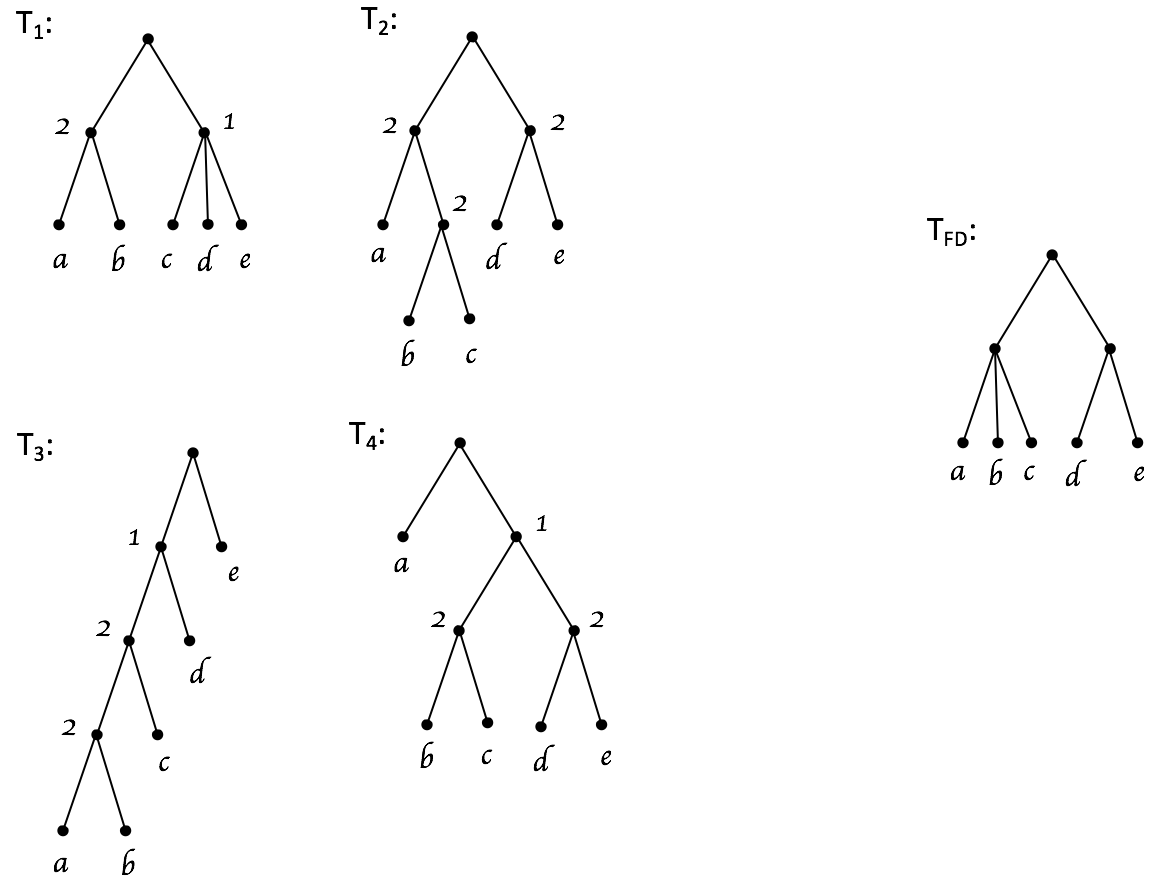
\includegraphics[scale=0.5]{freqdiff}
        \centering
        \caption{Let $\mathcal{S} = \{T_1, T_2, T_3, T_4\}$. $T_{FD}$ is the FDCT of $\mathcal{S}$. The number beside each non-root internal node $u$ indicates the weight of the node, $\weight(u)$, which is the number of occurences of the cluster $\leafset(u)$ in $\mathcal{S}$.}
        \label{fig:freqdiff}
    \end{figure}

    A \textit{frequency difference consensus tree} is defined as follows. Let $\mathcal{S}$ be a set of $k$ trees with identical leaf labels, i.e. $\mathcal{S} = \{T_1, T_2, ..., T_k\}$, where $\leafset(T_1) = \leafset(T_2) = ... = \leafset(T_k) = L$. For any cluster $C \subseteq L$, let weight of $C$, denoted as $\weight(C)$, be $|\{T : T \in \mathcal{S} \text{ and } C \in \mathcal{C}(T)\}|$, i.e. the number of trees in $\mathcal{S}$ which $C$ occurs in. For convenience, we also define, for any tree $T \in \mathcal{S}$, for any node $u \in V(T)$, the weight of $u$, denoted as $\weight(u)$ to be $\weight(\leafset^{T}(u))$. Then the FDCT of $\mathcal{S}$ is the tree $T_{FD}$, where $\mathcal{C}(T_{FD}) = \{C : C \subseteq L \text{ and } \weight(C) > max(\{\weight(C_1) : C_1 \subseteq L \text{ and } C \not\compatible C_1\})\}$. Thus $T_{FD}$ contains all clusters that occur more frequently than any cluster that they are incompatible with. By Proposition $3$ in \cite{steel2014axiomatic}, this tree always exists and is unique for a given $\mathcal{S}$. Figure~\ref{fig:freqdiff} gives an example. In this, $\weight(\{a, b\}) = 2 \leq \weight(\{b, c\}) = 2$ and $\{a, b\} \not\compatible \{b, c\}$, hence $\{a, b\}$ is not in the final consensus tree. However $\{a, b, c\}$ and $\{d, e\}$ have frequencies greater than any cluster incompatible with them, hence they both exist in the consensus tree. Note that frequencies are not shown for the trivial clusters.

    For each of the definitions above where the tree is specified in the superscript, this superscript is omitted if the tree being referred to is clear from context. For example, $children^T(u)$ would be written as $children(u)$. This will also be applied to any notation developed in the remainder of this text.

    Henceforth, $\mathcal{S}$ is taken to be the input set of trees with identical leaf labels. This set of leaf labels is denoted by $L$. Let $|\mathcal{S}| = k$ and $|L| = n$.

    \subsection{Previous Work}
    An implementation of the FDCT can be found in the free software package TNT \cite{goloboff2008tnt}; however the algorithm used within is unavailable and so its complexity is not known. Jansson et al. \cite{jansson2018algorithms} gave a deterministic $min\{O(kn^2), O(kn(k + log^2 n))\}$ algorithm for constructing the FDCT, implemented in the open source FACT package \cite{jansson2016improved}. Gawrychowski et al. \cite{gawrychowski2017faster} improved upon this to give a deterministic $O(kn\,log^2n)$ algorithm (not yet implemented).

    \subsection{Organisation of the Article and New Results}
    Section~\ref{sec:preliminaries} contains some results from previous works that are utilised later. Sections~\ref{sec:cfd} and~\ref{sec:rmqtree} show how certain efficient data structures can be built on trees; these will be utilised later. Sections~\ref{sec:weighting} and~\ref{sec:filterclusters} present algorithms for solving subproblems of the FDCT construction; these are brought together in \ref{sec:freqdiffconstruction} to give a new deterministic algorithm for constructing the FDCT that runs in $O(kn\,log\,n)$ time.

    \section{Preliminaries}
    \label{sec:preliminaries}

    \subsection{The \textit{lca} operation}

    We restate the following lemma outlining the \textit{lca} operation from \cite{bender2000lca}:
    \newline

    \begin{lca}
        \label{lem:lca}

        Given any tree $T$, the $lca$ data structure can be constructed in $O(n)$ time, where $n = |V(T)|$. Then, for any nodes $u, v \in V(T)$, the query $lca^{T}(u, v)$ can be answered in constant time.
    \end{lca}

    \subsection{The linear RMQ (range minimum/maximum) data structure}

    For any array $A[1 ... n]$ of length $n$ and any indices $i, j$, $1 \leq i \leq j \leq n$, let $rmq^A(i, j)$ denote $max_{i \leq k \leq j}A[k]$. We restate the following lemma about answering $rmq$ queries from \cite{bender2000lca}:
    \newline

    \begin{linearrmq}
        \label{lem:linearrmq}

        Given an array $A$ of numbers of length $n$, the \textit{linear RMQ data structure} can be constructed in $O(n)$ preprocessing time. Then for any indices $i, j$, $1 \leq i \leq j \leq n$, the query $rmq^A(i, j)$ can be answered in constant time.
    \end{linearrmq}

    \subsection{Centroid Path Decomposition}

    The \textit{centroid path decomposition technique} of \cite{cole2000n} is used to decompose a tree $T$ into a path from the root to some leaf and a set of disjoint subtrees. For any $u \in V(T)$, we define the \textit{heaviest child} of $u$, denoted by $heavyChild(u)$, to be the one with the largest leafset, with ties broken arbitrarily. The remaining children are called the \textit{side children} of $u$, denoted by $sideChildren(u)$. A \textit{centroid path} in $T$ is the path formed by starting at the root and at each point following the heaviest child. The centroid path is denoted by $\pi(T) = \langle p_{\gamma}, p_{\gamma - 1}, ..., p_1 \rangle$, where $p_{\gamma}$ is the root of $T$ and $p_1$ is a leaf. Removing the path $\pi(T)$ from $T$ results in a set of disjoint subtrees of $T$, where the root of each such subtree is a child of some node in $\pi(T)$. These trees are called the \textit{side trees} of $\pi(T)$, denoted by $\sigma(T)$. Also, for any node $p_i \in \pi(T)$, let $\sigma(p_i)$ be the set of trees rooted at $sideChildren(p_i)$, called the side trees \textit{associated} with $p_i$. Figure~\ref{fig:centroid}(a) demonstrates this decomposition. Here, the bold path from the root to leaf is the centroid path. When the dashed edges and the nodes contained in the centroid path are removed from the tree, the side trees remain. In particular, it can be seen that there are two side trees associated with the root, one containing just a single leaf, while the other is a larger tree.

    We further define a \textit{complete centroid path decomposition} for any tree $T$. Here, the normal centroid path decomposition is applied on $T$, and then each side tree is recursively decomposed. This results in a set of disjoint paths in $T$, denoted by $\mathcal{P}(T)$. We also assign each path $P_i \in \mathcal{P}(T)$ a depth, denoted as $depth^{T}(P_i)$, defined to be $1\, +$ depth of centroid path containing the parent of the root of $P_i$. Intuitively, if we build a tree from only the roots of the centroid paths while maintaining the same relative structure, then the depth of a centroid path would simply be the depth of its root in this new tree. Figure~\ref{fig:centroid}(b) applies complete centroid path decomposition on the same tree as before. The bold paths, along with the isolated leaves, are centroid paths. As can be seen, the large side tree that remained intact in Figure~\ref{fig:centroid}(a) has now been recursively decomposed. The depth of each centroid path is shown next to its root.

    \begin{figure}[h]
        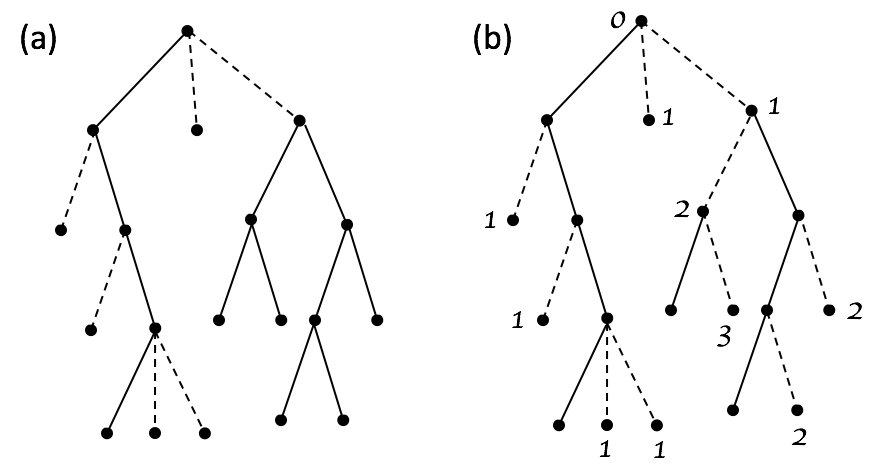
\includegraphics[scale=0.5]{centroid}
        \centering
        \caption{Demonstration of centroid path decomposition. Both (a) and (b) use the same tree. In (a), the tree has undergone a centroid path decomposition such that after the dashed edges are removed, leaving a centroid path and a set of side trees. In (b), the tree has undergone a complete centroid path decomposition, with the dashed edges being removed to leave only a set of paths. The depth of each centroid path is shown next to its root.}
        \label{fig:centroid}
    \end{figure}

    \subsection{The \textit{delete} operation}
    \label{subsec:delete}

    As described in \cite{jansson2018algorithms}, the \textit{delete} operation deletes a cluster from a tree. To do so, we specify some internal node $u$ in a tree $T$, such that we wish to delete the cluster $\leafset^{T}(u)$. Then the \textit{delete} operation makes $parent(u)$ the parent of all nodes in $children(u)$ and removes $u$, along with any associated edges from $T$. This has the effect of removing only $\leafset(u)$ from $T$, without affecting any other cluster. For example, in Figure~\ref{fig:freqdiff}, if we perform a delete operation on $T_2$, on the node associated with the cluster $\{b, c\}$, the resulting tree is identical to $T_{FD}$.

    \subsection{Characterising incompatibility}

    We restate Lemma 6 of \cite{jansson2018algorithms} here since it is crucial in the development of an algorithm discussed below:
    \newline

    \begin{incompatibility}
        \label{lem:incompatibility}

        Given a tree $T$ and a cluster $C \subseteq \leafset(T)$, let $l_C = lca^T(C)$. Then for any $u \in V(T)$, $C \not\compatible \leafset(u)$ iff $u$ lies on the path between $l_C$ and some $x \in C$ and $\leafset(u) \not\subseteq C$.
    \end{incompatibility}

    \subsection{The \texttt{Merge\_Trees} algorithm}
    \label{subsec:mergetrees}

    We restate the following lemma outlining the \texttt{Merge\_Trees} operation from \cite{jansson2016improved}:
    \newline

    \begin{mergetrees}
        \label{lem:mergetrees}

        Given trees $T_1$ and $T_2$ where $\leafset^{T_1} = \leafset^{T_2} = L$ and $T_1 \compatible T_2$, \texttt{Merge\_Trees}$(T_1, T_2) = T$, where $\leafset^T = L$ and $\mathcal{C}(T) = \mathcal{C}(T_1) \cup \mathcal{C}(T_2)$. This algorithm runs in $O(|L|)$ time.
    \end{mergetrees}

    \begin{figure}[h]
        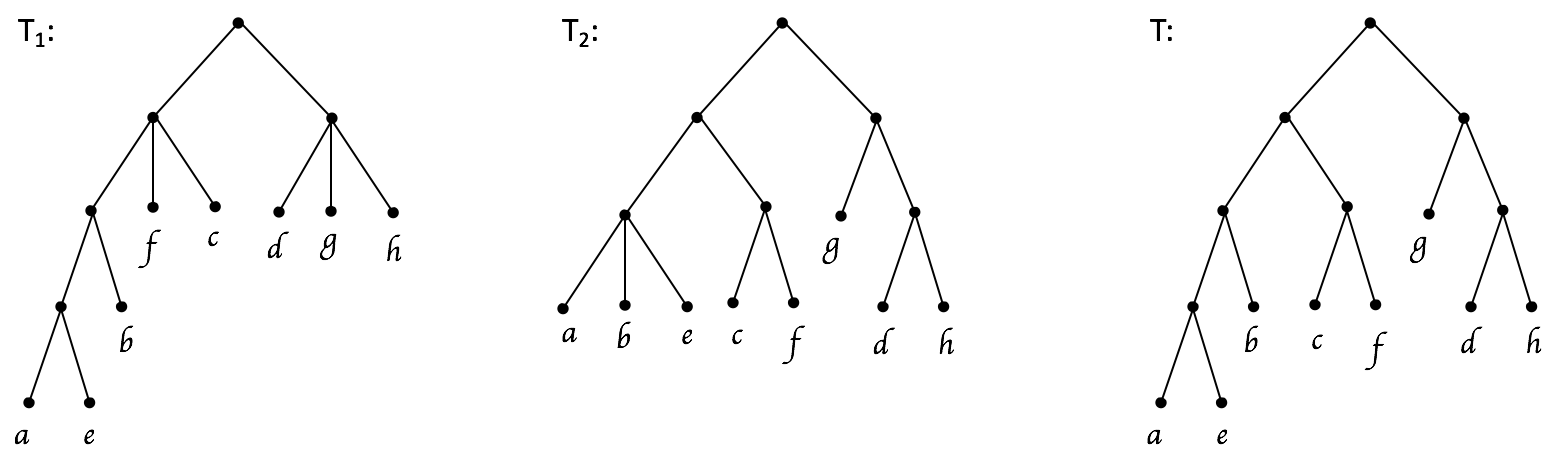
\includegraphics[scale=0.5]{mergetrees}
        \centering
        \caption{$T_1 \compatible T_2$. $T =$ \texttt{Merge\_Trees}$(T_1, T_2)$. $\mathcal{C}(T) = \mathcal{C}(T_1) \cup \mathcal{C}(T_2)$.}
        \label{fig:mergetrees}
    \end{figure}

    Figure~\ref{fig:mergetrees} gives an example for the \texttt{Merge\_Trees} algorithm. Here, $T_1 \compatible T_2$ and $T =$ \texttt{Merge\_Trees}$(T_1, T_2)$. Observe that,
    \begin{align*}
        \mathcal{C}(T_1) &= \{\{a, e\}, \{a, b, e\}, \{a, b, c, e, f\}, \{d, g, h\}\}\\
        \mathcal{C}(T_2) &= \{\{a, b, e\}, \{c, f\}, \{a, b, c, e, f\}, \{d, h\}, \{d, g, h\}\}\\
        \mathcal{C}(T) &= \{\{a, e\}, \{a, b, e\}, \{c, f\}, \{a, b, c, e, f\}, \{d, h\}, \{d, g, h\}\}\\
        &= \mathcal{C}(T_1) \cup \mathcal{C}(T_2).
    \end{align*}

    \subsection{The \texttt{Frequency\_Difference} algorithm}

    The algorithm \texttt{Frequency\_Difference} \cite{jansson2018algorithms} computes the FDCT of a set of trees $\mathcal{S}$. It runs in two parts. First, for any tree $T \in \mathcal{S}$ and any node $u \in V(T)$, it computes $\weight(u)$ in the \textit{weighting} step. In the second part, it utilises \texttt{Filter\_Clusters} (defined below) and \texttt{Merge\_Trees} (from Subsection~\ref{subsec:mergetrees}) to compute the FDCT.

    As in \cite{jansson2018algorithms}, the subprocedure \texttt{Filter\_Clusters}, is defined to take as input trees $\TA$ and $\TB$, with $\leafset^{\TA} = \leafset^{\TB} = L$ and the values of $\weight(u)$ for all $u \in V(\TA) \cup V(\TB)$. It returns a tree $T$ which contains all clusters $C$ in $\TA$ for which $\weight(C) > $ weights of all clusters in $\TB$ that are incompatible with $C$. Formally, \texttt{Filter\_Clusters}$(\TA, \TB) = T$ where $\mathcal{C}(T) = \{C : C \in \mathcal{C}(\TA) \text{ and } \weight(C) > max(\{\weight(C_1) : C_1 \in \mathcal{C}(\TB) \text{ and } C_1 \not\compatible C\})\}$ and $\leafset^T = L$. For example, referring to Figure~\ref{fig:freqdiff}, \texttt{Filter\_Clusters}$(T_2, T_1) = T_{FD}$. Notice that there are three non-trivial clusters in $T_2$: $\{a, b, c\}, \{b, c\}$ and $\{d, e\}$. All of these have weight $2$. Now the only cluster in $T_1$ incompatible with $\{a, b, c\}$ is $\{c, d, e\}$, but this only has weight $1$ and so $\{a, b, c\}$ is kept. The cluster $\{d, e\}$ is compatible with $T_1$ so it is also kept. However, $\{b, c\}$ is incompatible with $\{a, b\}$ and they both have weight $2$, hence $\{b, c\} \not\in \mathcal{C}($\texttt{Filter\_Clusters}$(T_2, T_1))$.

    The \texttt{Frequency\_Difference} algorithm is given below.

    \begin{algorithm}
        \caption{Frequency\_Difference}
        \label{alg:frequencydifference}

        \begin{algorithmic}[1]
            \Input A set $\mathcal{S}$ of trees $\{T_1, T_2, ..., T_k\}$ where $\leafset(T_1) = \leafset(T_2) = ... = \leafset(T_k) = L$

            \Output A tree $T_{FD}$, where $\mathcal{C}(T_{FD}) = \{C : C \subseteq L \text{ and } \weight(C) > max(\{\weight(C_1) : C_1 \subseteq L \text{ and } C \not\compatible C_1\})\}$ and $\leafset^{T_{FD}} = L$.

            \State Compute $\weight(C)$ for every cluster $C$ that occurs in $S$.

            \State $T := T_1$

            \For{$j := 2$ to $k$}
                \State $A :=$ \texttt{Filter\_Clusters}$(T, T_j)$

                \State $B :=$ \texttt{Filter\_Clusters}$(T_j, T)$

                \State $T :=$ \texttt{Filter\_Clusters}$(A, B)$
            \EndFor

            \For{$j := 1$ to $k$}
                \State $T :=$ \texttt{Filter\_Clusters}$(T, T_j)$
            \EndFor

            \State \Return $T$
        \end{algorithmic}
    \end{algorithm}

    Theorem 3 of \cite{jansson2018algorithms} gives the following corollary:
    \newline

    \begin{freqdiffruntimecomponents}
        \label{cor:freqdiffruntimecomponents}

        The total runtime of \texttt{Frequency\_Difference} is given by $O(g(n, k) + k \cdot f(n))$ where $g(n, k)$ is the time taken by the weighting step and $f(n)$ is the runtime of \texttt{Filter\_Clusters}.
    \end{freqdiffruntimecomponents}

    Jansson et al. \cite{jansson2018algorithms} gave a $min(\{O(kn^2), O(k^2n)\})$ solution to the weighting step and an $O(n\,log^2n)$ solution to \texttt{Filter\_Clusters}, giving an overall runtime of $min(\{O(kn^2), O(kn(k + log^2n))\})$. Gawrychowski et al. \cite{gawrychowski2017faster} improved the runtime of the weighting step to $O(kn\,log^2n)$, thus reducing the overall runtime to $O(kn\,log^2n)$.

    \section{$childD$ queries}
    \label{sec:cfd}

    Given a tree $T$ and nodes $v, w \in V(T)$ such that $w$ is a proper ancestor of $v$, define $childD(v, w)$ as the child of $w$ that is an ancestor of $v$. We construct a data structure that allows us to answer this query in constant time, given $O(n\,log\,n)$ preprocessing time, where $n = |V(T)|$.

    Reorder $T$ such that the heaviest child of each node is its leftmost child. Then the leaves of $T$ are indexed in left to right order, such that every leaf $x \in \leafset^T$ is assigned a value $index(x)$. Then for every node $u \in V(T)$, the indices of the leaves in $T[u]$ form a consecutive range. For each internal node $u \in V(T)$, define its side children to be the set $children(u) - \{\text{heaviest child of }u\}$ and its side trees to be the subtrees of $T$ rooted at its side children. Let $x$ and $y$ be the leaves in the side trees of $u$ with the smallest and largest indices respectively. We now build the array $cFL_u[0\, ...\, index(y) - index(x)]$ which maps each leaf $z$ in the side trees of $u$ to the child of $u$ that is an ancestor of $z$. Thus, for every leaf $z$ in $T[v]$ for some $v \in$ side children of $u$, let $cFL_u[index(z) - index(x)] = v$.
    \newline

    \begin{cfddatastructure}
        \label{lem:cfddatastructure}

        Given a tree $T$ where $n = |V(T)|$, the $cFL$ data structure defined above can be constructed in $O(n\,log\,n)$ time.

        \begin{proof}
            Rearranging $T$ and indexing the leaves can be done in two $O(n)$ passes. By the standard argument of centroid-path decomposition, we argue that any leaf is in the side trees of $O(log\,n)$ nodes, hence the total size of the $cFL$ arrays is $O(n\,log\,n)$. It is easy to see that these arrays can thus be constructed in $O(n\,log\,n)$ time.
        \end{proof}
    \end{cfddatastructure}

    \medskip
    \begin{cfdquery}
        \label{lem:cfdquery}

        Given a tree $T$, an $lca$ data structure on $T$, the $cFL$ data structure on $T$ and nodes $v, w \in V(T)$, the query $childD(v, w)$ can be answered in constant time.

        \begin{proof}
            The query is divided into two parts. First, we check if $v$ is a descendant of the heaviest child of $w$. If so, we are done. If not, we need to determine which child of $w$ is an ancestor of $v$.

            To answer the first part, we can see that, given nodes $r, s \in V(T)$, $s$ is an ancestor of $r$ iff $lca(r, s) = s$. Thus we can check if $v$ is a descendant of the heaviest child of $w$ in $O(1)$ time since by Lemma~\ref{lem:lca}, the $lca$ data structure allows queries in constant time.

            For the second part, we simply retrieve the entry corresponding to any leaf in $\leafset(v)$ from $cFL_w$, again easily done in constant time.
        \end{proof}
    \end{cfdquery}

    \section{RMQ structure on trees}
    \label{sec:rmqtree}

    Here, we generalise the linear RMQ data structure to trees. Given a tree $T$ and $\weight(u)$ for each $u \in V(T)$, for any nodes $v, w \in V(T)$ such that $w$ is an ancestor of $v$, let $rmqTree^T[v, w] = max_{u \in path^T[v, w]}\weight(u)$. Note that the square brackets are again used to indicate inclusion of the two endpoints. We build a data structure for answering $rmqTree^T[v, w]$ queries in constant time, given $O(n\,log\,n)$ preprocessing time, where $n = |V(T)|$.

    The data structure outlined here builds on the one presented in Lemma 8 of \cite{jansson2018algorithms}, while providing some further details of the implementation. We do a complete centroid path decomposition on $T$. Then for each leaf $x \in \leafset^T$, the path from $x$ to the root of $T$ can be seen as a concatenation of subpaths of centroid paths in $\mathcal{P}(T)$. An example of this can be seen in Figure~\ref{fig:rmq}. This figure shows part of a tree. The diagonal lines from right to left are centroid paths in the tree (elements of $\mathcal{P}(T)$). The dashed edges indicate that the child is not the heaviest child of its parent, hence starting a new centroid path. As can be seen, the path from the leaf $x$ to the root consists of subpaths of many centroid paths. The data structure we build consists of two parts. Firstly, for each centroid path $P_i \in \mathcal{P}(T)$, the weights along $P_i$ are stored in a linear RMQ structure (as described in Lemma~\ref{lem:linearrmq}). Secondly, for each $x$, we denote the subpaths of centroid paths on the leaf-root path by $Q_1, Q_2, ..., Q_f$, where $Q_1$ contains $root(T)$ and $Q_f$ contains $x$. Then we build the array $W_x[1 ... f]$, where $W_x[i] = max_{u \in Q_i} \weight(u)$ and store this array in a linear RMQ structure.
    \newline

    \begin{figure}[h]
        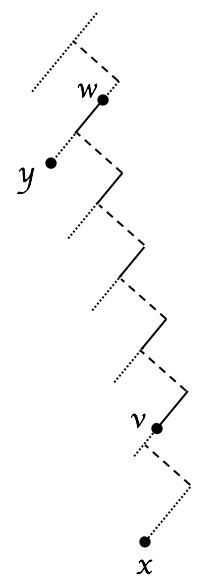
\includegraphics[scale=0.5]{rmq}
        \centering
        \caption{Demonstration of an $rmqTree[v, w]$ query. The diagonal lines from right to left are centroid paths of the tree. The parts in bold lie on the path between $v$ and $w$, while those that are dotted do not. Dashed lines connect the root of a centroid path to its parent. $y$ is the leaf at the bottom of the centroid path to which $w$ belongs. $x$ is some leaf in the subtree rooted at $v$.}
        \label{fig:rmq}
    \end{figure}

    \begin{rmqdatastructure}
        \label{lem:rmqdatastructure}

        Given a tree $T$ and $\weight(u)$ for each $u \in V(T)$, the $rmqTree$ data structure can be built in $O(n\,log\,n)$ time.

        \begin{proof}
            The decomposition step, along with computation of depths for nodes and for centroid paths can be done in $O(n)$ time. Storing the centroid paths in linear RMQ structures takes $O(n)$ time, by Lemma~\ref{lem:linearrmq} and since the total size of the centroid paths is $O(n)$. By the standard argument of centroid-path decomposition, it can be seen that for each leaf $x$, the number of centroid subpaths on the path from the leaf to the root of $T$ is $O(log\,n)$. Hence it takes $O(log\,n)$ time to build the linear RMQ structure for these subpaths. Since there are $n$ leaves, the total time taken to construct the linear RMQ structures for all leaves is $O(n\,log\,n)$.
        \end{proof}
    \end{rmqdatastructure}

    \medskip
    \begin{rmqquery}
        \label{lem:rmqquery}

        Given a tree $T$, an $lca$ data structure on $T$, the $rmqTree$ data structure on $T$, and nodes $v, w \in V(T)$ such that $w$ is an ancestor of $v$, the query $rmqTree[v, w]$ can be answered in constant time.

        \begin{proof}
            We use the complete centroid path decomposition done when producing the $rmqTree$ data structure. The path from $v$ to $w$ is partitioned into a concatenation of subpaths of these centroid paths, denoted by $Q_1, Q_2, ..., Q_g$. This is illustrated in Figure~\ref{fig:rmq}. The diagonal lines from right to left are some of the centroid paths the tree has been decomposed into. The dashed edges indicate that the child is not the heaviest child of its parent, such that the child is the root of a new centroid path. The bold lines are the subpaths of centroid paths that lie on the path from $v$ to $w$. $Q_1$ is the bold centroid subpath starting from $v$ and continuing upwards till the root of that path. Similarly, $Q_g$ is the bold centroid subpath starting at $w$ and continuing downwards until the path splits from that centroid path. $Q_2$ to $Q_{g - 1}$ are the bold centroid subpaths between $Q_1$ and $Q_g$. The significance of the leaves $x$ and $y$ is explained below.

            Take any $x \in \leafset(v)$. Then $Q_2, ..., Q_{g - 1}$ are contained fully in the centroid subpaths on the path from $x$ to the root of $T$. $Q_1$ must be a subpath that starts at $v$ in some centroid path $\in \mathcal{P}(T)$ and ends at the root of that centroid path. $Q_g$ is a subpath that starts at some node in some centroid path $\in \mathcal{P}(T)$ and ends at $w$, within the same path. We address each of these three divisions separately.

            To find the maximum weight within $Q_1$, we obtain the depth of $v$ within $Q_1$ by subtracting the depth of the root of $Q_1$ from the depth of $v$. Then the maximum weight can be retrieved by querying the linear RMQ structure for this centroid path, from the root to $v$ (recall that the depths and linear RMQ structures were obtained while constructing the $rmqTree$ data structure). Querying the linear RMQ structure costs constant time, as set out in Lemma~\ref{lem:linearrmq}.

            To find the maximum weight for the subpaths $Q_2, ..., Q_{g - 1}$, we obtain the indices of $Q_2$ and $Q_{g-1}$ in $W_x$ as $depth^{T}(Q_1) + 1$ and $depth^{T}(Q_g) - 1$ respectively. The maximum weight can then be found by querying $W_x$.

            Finally, we need to find the maximum weight within $Q_g$. Observe that the key here is finding which node is at the end of $Q_g$. Let $P_i \in \mathcal{P}(T)$ be the centroid path of which $Q_g$ is a subpath. Then the previous question is equivalent to finding which node in $P_i$ has $v$ in one of its side trees. Let $y$ be the leaf at the bottom of $P_i$. Then the desired node is simply $lca(y, v)$, querying for which takes $O(1)$ time as given by Lemma~\ref{lem:lca}. The maximum weight within $Q_g$ can now be easily found in constant time by querying the linear RMQ structure for $P_i$, from $w$ to $lca(y, v)$.

            As of these three values can be obtained in constant time, the query as a whole takes $O(1)$ time.
        \end{proof}
    \end{rmqquery}

    \section{Weighting}
    \label{sec:weighting}

    Given the set of trees $\mathcal{S} = \{T_1, T_2, ..., T_k\}$, where $\leafset(T_1) = \leafset(T_2) = ... = \leafset(T_k) = L$ and $n = |L|$, the weighting step computes $\weight(u)$ for every node $u \in \bigcup_{T \in \mathcal{S}}V(T)$. Recall that $\weight(u)$ gives the frequency of $\leafset(u)$ in $\mathcal{S}$. We divide this work (as in \cite{gawrychowski2017faster}) into the labelling and counting steps. The labelling step assigns a label to each node $u \in T, T \in \mathcal{S}$, denoted by $id(u)$, such that $id(u) \in [1 ... 2kn]$ and for any node $u' \in T', T' \in \mathcal{S}$, $id(u) = id(u')$ iff $\leafset^T(u) = \leafset^{T'}(u')$. That is, two nodes have the same label iff they are associated with the same cluster. The counting step sorts these labels, allowing us to count how many nodes exist with each label, giving us the frequencies (or the weights) of the nodes.

    Recall that the approach in \cite{gawrychowski2017faster} costs $O(kn\,log^2n)$ time. We develop a way to achieve $O(kn\,log\,n)$ time.

    The idea here will be to divide $L$ into two equal sized halves, $L'$ and $L''$. Then, we wish to build the sets $\{\leafset^T(u) \cap L' : T \in \mathcal{S}, u \in V(T)\}$ and $\{\leafset^T(u) \cap L'' : T \in \mathcal{S}, u \in V(T)\}$. If each of these sets could be labelled such that each cluster within them has a unique label, then for any tree $T \in \mathcal{S}$, for any node $u \in V(T)$, $\leafset^T(u)$ is uniquely identified by the pair $(id(\leafset^T(u) \cap L'), id(\leafset^T(u) \cap L''))$. To be able to achieve this, we introduce the definitions below.

    First, for any tree $T$ and any cluster $C \subseteq \leafset(T)$, define $T|C$, read as ``$T$ restricted to $C$'', as the tree $T'$ with $V(T') = \{lca^T(u, v) : u, v \in C\}$ which obeys $lca^T(C') = lca^{T'}(C')$ for all $C' \subseteq C$. Intuitively, $T'$ has the leaf set $C$ and consists of all nodes in $T$ that are $lca$'s of the leaves in $C$, with these nodes connected such that they have the same ancestor/descendant relationships as they had in $T$. Figure~\ref{fig:labelclusters} demonstrates this process; the tree $T_1|L'$ is $T_1$ restricted to the cluster $\{a, b, c, d\}$. Notice that nodes which are not $lca$'s of these leaves are removed, but the structure of the tree in relation to these leaves remains the same.

    Further, for every cluster $C \subseteq L$, and every node $u$ in $T$, define the node $assoc^C(u) = lca^T(C \cap \leafset^T(u))$. Notice that if $C \cap \leafset^T(u) \neq \emptyset$, $assoc^C(u) \in V(T|C)$ since it is the $lca$ of some non-empty subset of $C$. However, if $C \cap \leafset^T(u) = \emptyset$, then for convenience let $assoc^{C}(u) = \Phi$, where $\Phi$ is a special node with $id(\Phi) = 0$ and $\leafset(\Phi) = \emptyset$. We refer to Figure~\ref{fig:labelclusters} to show examples of this concept. Let $u$ and $v$ be the nodes in $T_1$ labelled $(5, 1)$ and $(5, 0)$ respectively. Then $assoc^{\{a, b, c, d\}}(u) = v$, since $v = lca^{T_1}(\{a, b, c, d\} \cap \leafset^{T_1}(u)) = lca^{T_1}(\{a, b\})$. $assoc^{\{e, f, g, h\}}(v) = \Phi$, since $\leafset^{T_1}(v) \cap \{e, f, g, h\} = \emptyset$.

    Using these observations, we can expand on the previous description of the algorithm. We divide $L$ into $L'$ and $L''$, then we construct and recursively label the sets $\{T|L' : T \in \mathcal{S}\}$ and $\{T|L'' : T \in \mathcal{S}\}$. Then for any tree $T \in \mathcal{S}$, for any node $u \in V(T)$, $\leafset^T(u)$ can be represented by the pair $(id(assoc^{L'}(u)), id(assoc^{L''}(u)))$. Once we obtain these pairs, we sort them and assign a rank to each unique pair; $id(u)$ is then the rank of the pair $(id(assoc^{L'}(u)), id(assoc^{L''}(u)))$. The resulting algorithm \texttt{Label\_Clusters} is laid out below.

    \begin{algorithm}
        \caption{Label\_Clusters}
        \label{alg:labelclusters}

        \begin{algorithmic}[1]
            \Input A set $\mathcal{S}$ of trees $\{T_1, T_2, ..., T_k\}$ where $\leafset(T_1) = \leafset(T_2) = ... = \leafset(T_k) = L$

            \Output Associate a label $id(u) \in [1 ... 2k |L|]$ with every node $u$ in the trees in $\mathcal{S}$ such that for any two nodes $v, w$ in some trees in $\mathcal{S}$, $id(v) = id(w)$ iff $\leafset(v) = \leafset(w)$.

            \State Partition $L$ into $L'$ and $L''$ such that $|L'| = |L''|$.

            \State For all $i \in [1 ... k]$, let $T'_i = T_i|L'$ and $T''_i = T_i|L''$.

            \State \texttt{Label\_Clusters}$(\{T'_1, T'_2, ..., T'_k\})$.

            \State \texttt{Label\_Clusters}$(\{T''_1, T''_2, ..., T''_k\})$.

            \State For every tree $T \in \mathcal{S}$, for every node $u \in T$, represent $u$ by the pair $(id(assoc^{L'}(u)), id(assoc^{L''}(u)))$.

            \State Radix sort all pairs obtained and remove duplicates. Assign a rank to each unique pair.

            \State For every tree $T \in \mathcal{S}$, for every node $u \in T$, set $id(u) = $ rank of the pair $(id(assoc^{L'}(u)), id(assoc^{L''}(u)))$.
        \end{algorithmic}
    \end{algorithm}

    One iteration of this process is illustrated in Figure~\ref{fig:labelclusters}. Here $L' = \{a, b, c, d\}$ and $L'' = \{e, f, g, h\}$. It is assumed that the algorithm has correctly labelled the clusters for each of the restricted trees, and these labels are assigned as shown in Figure~\ref{fig:labelclusters}(b). Figure~\ref{fig:labelclusters}(a) then shows the pair associated with each internal node of $T_1$ and $T_2$. For example, the cluster $\{a, b, e\}$ in $T_1$ is labelled by $5$ from $\{a, b\}$ in $T_1|L'$ and $1$ from $\{e\}$ in $T_1|L''$. Similarly, the cluster $\{a, b\}$ in $T_1$ is labelled by $5$ from $\{a, b\}$ in $T_1|L'$ and $0$ from $\Phi$ since $\{a, b\} \cap \{e, f, g, h\} = \emptyset$.

    \begin{figure}[h]
        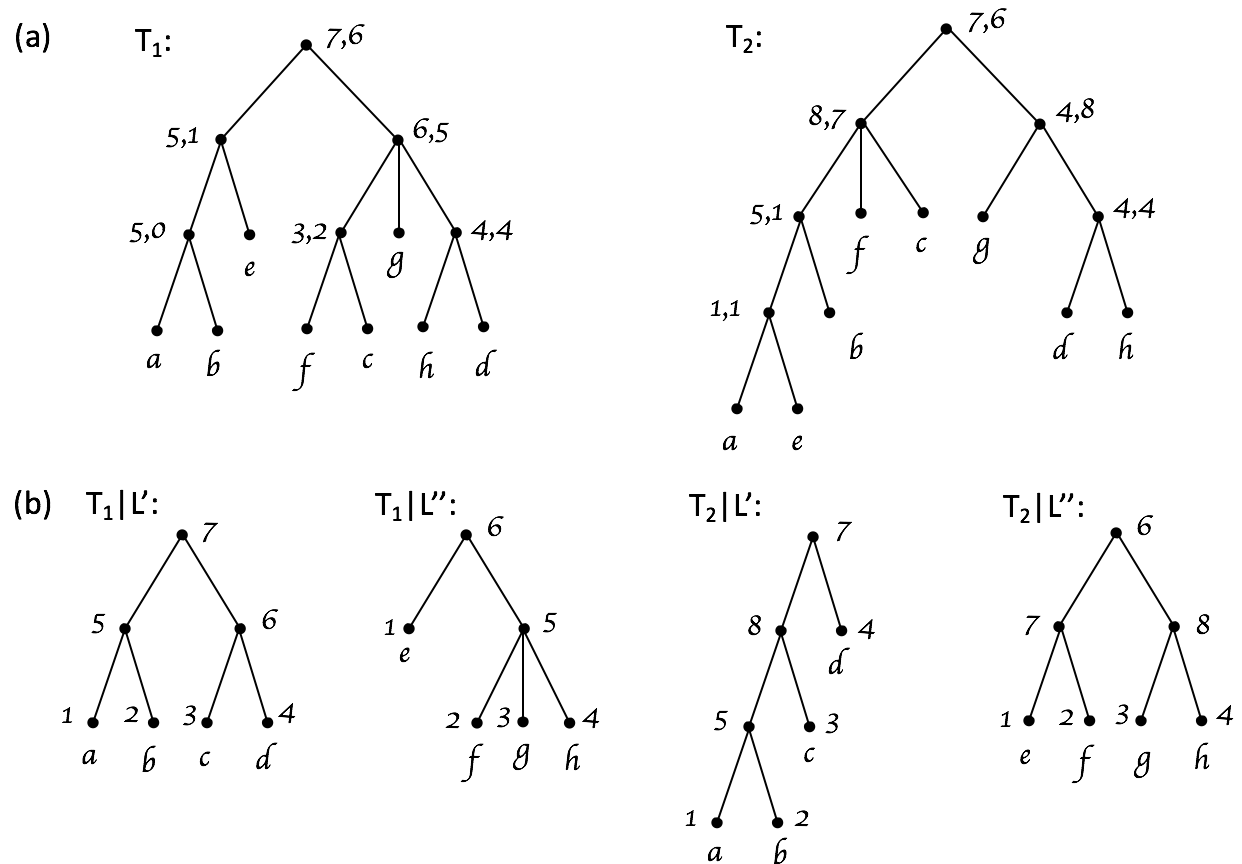
\includegraphics[scale=0.5]{labelclusters}
        \centering
        \caption{Demonstration of \texttt{Label\_Clusters}$(T_1, T_2)$. $L' = \{a, b, c, d\}$ and $L'' = \{e, f, g, h\}$. (b) shows the trees $T_1|L', T_1|L'', T_2|L'$ and $T_2|L''$, where these have been recursively labelled. The labels are shown beside each of the nodes. (a) shows the trees $T_1$ and $T_2$ where the pair that represents each node (except the leaves) is shown beside it.}
        \label{fig:labelclusters}
    \end{figure}

    {\color{red} I removed the shallowest descendant part completely, under the assumption that the process by which $assoc^C(u)$ is obtained is not hard to come up with. Is this reasonable, or should I prove something like $assoc^C(u) = $ shallowest descendant of $u$ in $T|C$?}

    The following Lemma proves the correctness of the given algorithm:

    \bigskip
    \begin{labelclusterscorrectness}
        \label{lem:labelclusterscorrectness}

        After running \texttt{Label\_Clusters}$(\mathcal{S})$, for any trees $T_i, T_j \in \mathcal{S}$, for any nodes $u \in V(T_i), v \in V(T_j)$, $id(u) = id(v)$ iff $\leafset^{T_i}(u) = \leafset^{T_j}(v)$.

        \begin{proof}
            $id(u) = id(v)$ iff $id(assoc^{L'}(u)) = id(assoc^{L'}(v))$ and $id(assoc^{L''}(u)) = id(assoc^{L''}(v))$. Inductively, $id(assoc^{L'}(u)) = id(assoc^{L'}(v))$ iff $\leafset^{T_i|L'}(assoc^{L'}(u)) = \leafset^{T_j|L'}(assoc^{L'}(v))$. By definition of the $assoc$ relation, $\leafset^{T_i}(u)\, \cap\, L' = \leafset^{T_j}(v)\, \cap\, L'$. Symmetrically, $id(assoc^{L''}(u)) = id(assoc^{L''}(v))$ iff $\leafset^{T_i}(u)\, \cap\, L'' = \leafset^{T_j}(v)\, \cap\, L''$. Since $L'$ and $L''$ partition $L$, both parts are true iff $\leafset^{T_i}(u) = \leafset^{T_j}(v)$.
        \end{proof}
    \end{labelclusterscorrectness}

    \medskip
    \begin{labelclustersidbounds}
        \label{lem:labelclustersidbounds}

        After running \texttt{Label\_Clusters}$(\mathcal{S})$, for any node $u \in V(T), T \in \mathcal{S}$, $id(u) \in [1 ... 2k |L|]$.

        \begin{proof}
            It is easily seen that $|V(T)| < 2|L|$. Thus the total number of pairs is less than $2k|L|$. This also places an upper bound on the number of ids. Notice that $u$ cannot be labelled with $0$ since that is reserved for the special node.
        \end{proof}
    \end{labelclustersidbounds}

    \medskip
    \begin{labelclustersruntime}
        \label{lem:labelclustersruntime}

        The algorithm \texttt{Label\_Clusters}$(\mathcal{S})$ runs in $O(kn\,log\,n)$ time.

        \begin{proof}
            Let $T(m)$ be the runtime of \texttt{Label\_Clusters}$(\mathcal{T})$, where $m =$ size of leaf set of each tree in $\mathcal{T}$. By Lemma 5.2 of \cite{farach1995fast}, construction of $T'_i$ and $T''_i$ takes $O(m)$ time for each $T_i \in \mathcal{T}$, taking total $O(km)$ time over all the trees. Computing $assoc^{L'}(u)$ and $assoc^{L''}(u)$ for each node $u$ in some tree $T_i \in \mathcal{T}$ can be done by a bottom up traversal of $T_i$ along with $T'_i$ and $T''_i$, taking $O(km)$ time total. Also observe that the number of pairs obtained is $O(km)$. Further, each of the values in the pair is in the range [0, km]. Thus radix sorting these pairs and assigning labels back to the nodes takes $O(km)$ time. So $T(m) = 2T(m/2) + O(km)$, giving $T(n) = kn\,log\,n$.
        \end{proof}
    \end{labelclustersruntime}

    \medskip
    \begin{weightingruntime}
        \label{lem:weightingruntime}

        The weighting step can be completed in $O(kn\,log\,n)$ time.

        \begin{proof}
            As shown in Lemma~\ref{lem:labelclustersruntime}, assigning labels to each node takes $O(kn\,log\,n)$ time. Next, we sort the labels by counting sort. Since each label is in the range $[1 ... 2kn]$ and there are $O(kn)$ labels, this takes $O(kn)$ time. The frequencies, or weights, can then be computed in $O(kn)$ time.
        \end{proof}
    \end{weightingruntime}

    \section{\texttt{Filter\_Clusters}}
    \label{sec:filterclusters}

    Given the trees $\TA$ and $\TB$ where $\leafset^{\TA} = \leafset^{\TB} = L$ and $n = |L|$, the algorithm \texttt{Filter\_Clusters}$(\TA, \TB)$ returns a tree $T$, where $\mathcal{C}(T) = \{C : C \in \mathcal{C}(\TA) \text{ and } \weight(C) > max(\{\weight(C_1) : C_1 \in \mathcal{C}(\TB) \text{ and } C_1 \not\compatible C\})\}$ and $\leafset(T) = L$. Recall that the previous best known solution, as in \cite{jansson2018algorithms}, costs $O(kn\,log^2n)$ time; we present an $O(kn\,log\,n)$ solution.

    The key here is finding, for any node $u \in V(\TA)$, the set of nodes in $\TB$ that are incompatible with $u$, so that we can find the maximum weight of these. Then it is easy to figure out whether $u$ should be in $T$ or not.

    Subsection~\ref{subsec:mincover} presents an insight into the structure of the trees under consideration, later shown to be the key to decreasing the runtime of the algorithm. Subsection~\ref{subsec:redefiningincompatibility} uses this insight to give a stricter definition of incompatibility. We then use these in Subsection~\ref{subsec:filterclusters} to create the algorithm \texttt{Filter\_Clusters}. Finally, Subsections~\ref{subsec:addtocover} and~\ref{subsec:updateincompatible} prove two claims we make when analysing the runtime of \texttt{Filter\_Clusters}.

    \subsection{The concept of a \textit{minimum cover}}
    \label{subsec:mincover}

    Given a tree $T$ and a cluster $C \subseteq L$, define a set $S \subseteq V(T)$ to be a cover of $C$ in $T$ if $\bigcup_{u \in S} \leafset^{T}(u) = C$. Then we define the minimum cover of $C$ in $T$, denoted as $minCover^{T}(C)$, to be the smallest set $S$ such that $S$ is a cover of $C$. Note that this set is well defined for each cluster. For example, in the tree in Figure~\ref{fig:mincover}, the circled nodes give the minimum cover of $C = \{a, b, c, f, g, h\}$.

    \begin{figure}[h]
        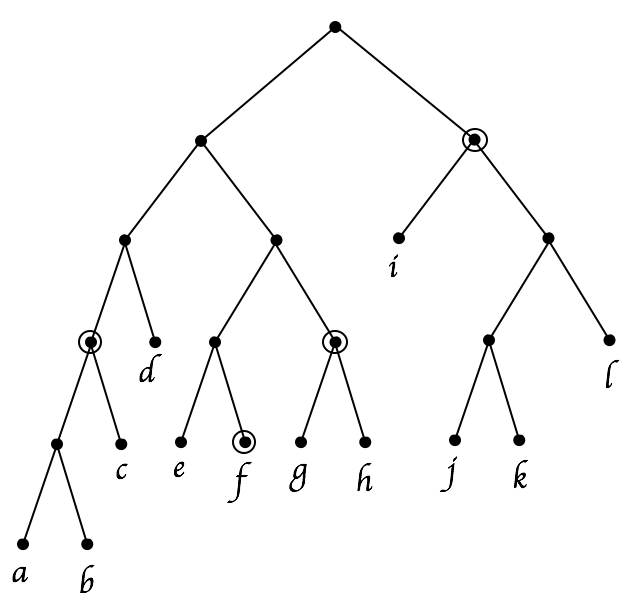
\includegraphics[scale=0.48]{mincover}
        \centering
        \caption{Illustration of a minimum cover and of Lemma~\ref{lem:mincoverrecursive}. Let $C = \{a, b, c, f, g, h\}$. Then the circled nodes in (a) give $minCover^{T}(C)$. Let $u$ be the leaf labelled with $e$, marked with a square in (a). We wish to execute $addToCover^{T}(minCover^{T}(C), u)$. (b) shows the state after one recursive call, where the circled nodes give the new minimum cover and the node marked with a square is the new $u$. (c) shows the state after the next (and last) recursive call, where the minimum cover of $C \cup \leafset^{T}(u)$ has been found to be the circled nodes.}
        \label{fig:mincover}
    \end{figure}

    \subsection{Redefining incompatibility}
    \label{subsec:redefiningincompatibility}

    With the concept of a minimum cover in hand, we can proceed to give a stricter definition of incompatibility. Given tree $T$ and cluster $C \subseteq L$, let the set $incompatible^{T}(C) = \{v : v \in V(\TB) \text{ and } \leafset^{\TB}(v) \not\compatible C\}$.
    \newline

    \begin{incompatibilitymincover}
        \label{lem:incompatibilitymincover}

        Given tree $T$ and cluster $C \subseteq L$, let $l_C = lca^{T}(C)$. Then for any node $u \in V(\TB)$, $u \in incompatible^{T}(C)$ iff $u$ is a proper ancestor of some node $c \in minCover^{T}(C)$ and $u$ is a proper descendant of $l_C$. In other words, $incompatible^{T}(C) = \bigcup_{c \in minCover^{T}(C)} path(c, l_C)$.

        \begin{proof}
            $\longrightarrow$. Given any $u \in V(T)$ such that $u \in incompatible^{T}(C)$, $u$ is a proper descendant of $l_C$ as a direct consequence of Lemma~\ref{lem:incompatibility}. Further, there is some leaf $x \in C$ such that $u$ is a proper ancestor of $x$ by Lemma~\ref{lem:incompatibility}. Then there must be some node $c \in V(T)$ such that $c$ is an ancestor of $x$ and $c \in minCover^{T}(C)$, otherwise $x$ would not be covered. If $c$ is an ancestor of $u$, then $\leafset^{T}(u) \subseteq \leafset^{T}(c) \subseteq C$, thus $\leafset^{T}(u) \compatible C$, which leads to a contradiction. Hence, $u$ is a proper ancestor of $c$.

            $\longleftarrow$. Given any $u \in V(T)$ such that $u$ is a proper ancestor of some node $c \in minCover^{T}(C)$ and $u$ is a proper descendant of $l_C$, $C \not\subseteq \leafset^{T}(u)$, since $u$ is a proper descendant of $l_C$. As $u$ is a proper ancestor of $c$, $\leafset^{T}(c) \subset \leafset^{T}(u)$. Also, $\leafset^{T}(c) \subset C$ by the definition of minimum cover. Thus $\leafset^{T}(u) \cap C \neq \emptyset$. Also, if $\leafset^{T}(u) \subseteq C$, we could create a smaller cover for $C$ by removing all proper descendants of $u$ from $minCover^{T}(C)$ and adding $u$. Note that this would give a smaller cover as there must be more than one such proper descendant of $u$, since $c$ is a proper descendant of $u$ and $\leafset^{T}(c) \subset C$. Hence, $u \in incompatible^{T}(C)$.
        \end{proof}
    \end{incompatibilitymincover}

    \begin{figure}[h]
        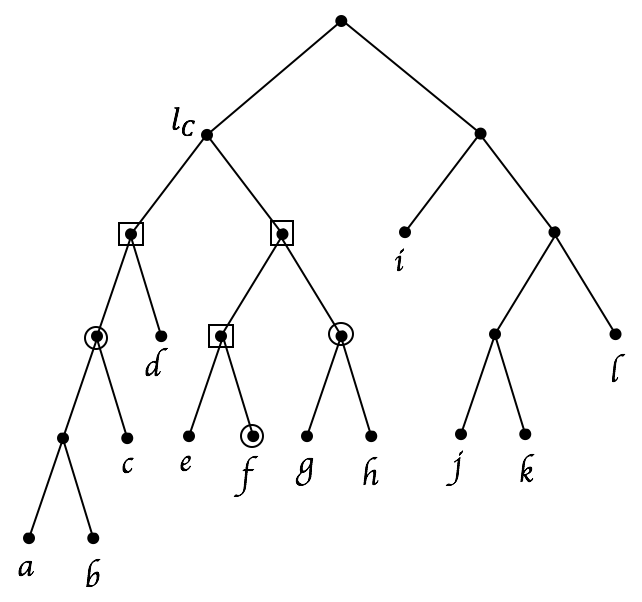
\includegraphics[scale=0.5]{incompatibility}
        \centering
        \caption{Illustration of Lemma~\ref{lem:incompatibilitymincover}. Let $C = \{a, b, c, f, g, h\}$. Then $l_C = lca^T(C)$, the circled nodes give $minCover^{T}(C)$ and the nodes marked with squared give $incompatible^T(C)$. Notice that all nodes in $incompatible^T(C)$ are proper descendants of $l_C$ are proper ancestors of some $c \in minCover^{T}(C)$.}
        \label{fig:incompatibility}
    \end{figure}

    The above result is illustrated in Figure~\ref{fig:incompatibility}.

    \subsection{The \texttt{Filter\_Clusters} algorithm}
    \label{subsec:filterclusters}

    Before going on to present \texttt{Filter\_Clusters} and analyse it, we make claims about the running time of an algorithm that finds the minimum cover and an algorithm that find incompatible nodes below. These are proved in Subsections~\ref{subsec:addtocover} and~\ref{subsec:updateincompatible} respectively.
    \newline

    \begin{mincoverruntime}
        \label{lem:mincoverruntime}

        Given a tree $T$, a cluster $C \subseteq L$ and a node $u \in V(T)$ such that $\leafset^{T}(u) \cap C = \emptyset$ let $S = minCover^{T}(C)$ and $Cu = C \cup \leafset^{T}(u)$. Then the operation $addToCover^{T}(S, u)$, which returns $minCover^{T}(Cu)$ and some node $v \in minCover^{T}(Cu)$ such that $v$ is an ancestor of $u$, can be performed in amortized $O(1)$ time.

        \begin{proof}
            Proved in Subsection~\ref{subsec:addtocover}.
        \end{proof}
    \end{mincoverruntime}

    \medskip
    \begin{incompatibilityruntime}
        \label{lem:incompatibilityruntime}

        Given a tree $T$, a cluster $C \subseteq L$ and a node $u \in V(T)$ such that $\leafset^{T}(u) \cap C = \emptyset$, let $S = minCover^{T}(C)$, $I = incompatible^{T}(C)$, $l_C = lca^{T}(C)$, $l_{Cu} = lca^{T}(C \cup \{u\})$ and $Cu = C \cup \leafset^{T}(u)$. Then the operation $updateIncompatible^{T}(S, I, u, l_C)$, which returns $(minCover^{T}(Cu), incompatible^{T}(Cu), l_{Cu})$, can be performed in amortized $O(1 + |incompatible^{T}(C) - incompatible^{T}(Cu)|\,\times\,log\,n)$, where $n = |\leafset^{T}|$.

        \begin{proof}
            Proved in Subsection~\ref{subsec:updateincompatible}.
        \end{proof}
    \end{incompatibilityruntime}

    With these operations in hand, we now develop the solution for \texttt{Filter\_Clusters}. Recall that this method takes trees $\TA$ and $\TB$ as input. First, for any node $u \in V(\TA)$, define $incompatible^{\TB}(u)$ to be $incompatible^{\TB}(\leafset^{\TA}(u))$. As discussed earlier, the idea is to find $incompatible^{\TB}(u)$ for each node $u \in V(\TA)$.

    \texttt{Filter\_Clusters} decomposes $\TA$ into a \textit{centroid path} and a set of \textit{side trees} (similarly to \cite{jansson2018algorithms}). Observe that for any side tree $\tau \in \sigma(\TA)$, $|\leafset^\tau| \leq n/2$ and that $\{\leafset^{\TA}(u) : \tau \in \sigma(\TA)\}$ forms a partition of $L\, \backslash\, {p_1}$. We further note that for any internal node $p_i \in \pi(\TA)$, $\leafset^{\TA}(p_{i - 1}) \subset \leafset^{\TA}(p_i)$, i.e. the cluster associated with $p_{i-1}$ is a proper subset of $p_i$. This then leads to the intuition behind the procedure \texttt{Filter\_Clusters} - recursively run the algorithm on the side trees, and then iterate over the centroid path from leaf to root. Here, for any non-leaf node $p_i \in \pi(\TA)$, we use
    the $addToCover$ and $updateIncompatible$ operations to find $incompatible^{\TB}(p_i)$.

    A key optimisation here is ensuring that when we call the function recursively on a side tree $\tau \in \sigma(\TA)$, the $\TB$ is restricted such that its leafset is the same as the leafset of $\tau$. Let $\tau$ be some side tree in $\sigma(\TA)$. We reuse the technique described in \cite{jansson2018algorithms} to construct a tree $\TB||\leafset^{\tau}$ such that $\leafset^{\TB||\leafset^{\tau}} = \leafset^{\tau}$, but at the same time does not lose important weight information. To do so, we first construct $\TB|\leafset^{\tau}$ and let the weight of each node in this tree be the same as its weight in $\TB$. For each non-root node $u \in V(\TB|\leafset^{\tau})$, let $v = parent^{\TB|\leafset^{\tau}}(u)$, then if $path^{\TB}(u, v) \neq \emptyset$, we create a new node $z$ in $\TB|\leafset^{\tau}$, set $parent(u) = z$ and $parent(z) = v$. Also, we set $\weight(z) = max_{w \in path^{\TB}(u, v)} \weight(w)$. Note that this value can be obtained with an $rmqTree^{\TB}[parent(u), cFD(v)]$ query, which we denote by $rmqTree^{\TB}(u, v)$. This gives us the tree $\TB||\leafset^{\tau}$.

    Further, for any node $u \in V(\TB||\leafset^{\tau})$, if $\leafset^{\TB||\leafset^{\tau}}(u) \neq \leafset^{\TB}(u)$, then $u$ is marked as $spoiled$. This concept is introduced since it will be important later to determine, for any node $u \in V(\TB||\leafset^{\tau})$, whether $\leafset^{\TB||\leafset^{\tau}}(u) \subseteq C$ for some cluster $C$. Special nodes are all marked as $spoiled$, since it is certain that the nodes they represent do not have their full leafset in $\TB||\leafset^{\tau}$. Observe that the ancestor of any spoiled node is also spoiled. Figure~\ref{fig:specialnodes} illustrates this entire process.

    \begin{figure}[h]
        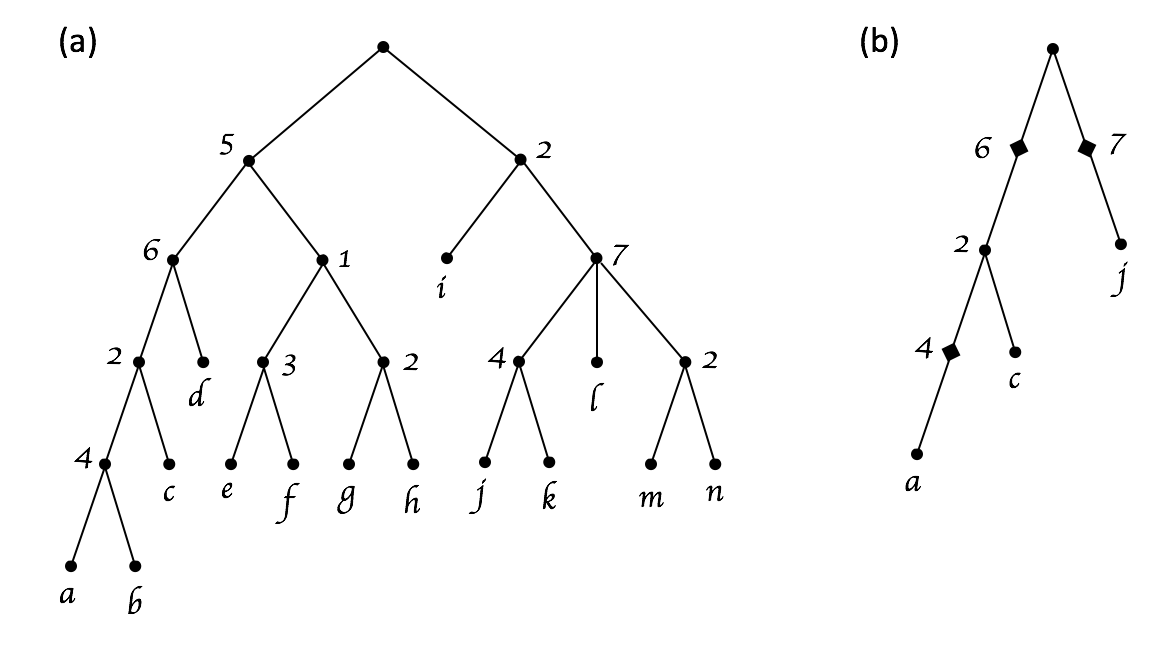
\includegraphics[scale=0.5]{specialnodes}
        \centering
        \caption{Part (a) shows a tree $T$ where all internal nodes are labelled with their weights. Part (b) shows the tree $T||\{a, c, j\}$. Again, internal nodes are labelled with their weights. Nodes represented by diamonds in this figure are special nodes. Observe that the special node that is a parent of the leaf $j$ has weight $7$ since the nodes on the path from $j$ to the root of $T$ had weights $4, 7$ and $2$. Also note that all internal nodes in (b) are spoiled.}
        \label{fig:specialnodes}
    \end{figure}

    In order to facilitate the $rmqTree$ queries, we preprocess $\TB$ to construct an RMQ and a cFD structure before \texttt{Filter\_Clusters} is called. Also note that we present a slightly modified version of \texttt{Filter\_Clusters} - rather than returning a tree $T$, where $\mathcal{C}(T) = \{C : C \in \mathcal{C}(\TA) \text{ and } \weight(C) > max(\{\weight(C_1) : C_1 \in \mathcal{C}(\TB) \text{ and } C_1 \not\compatible C\})\}$, it returns the set of nodes $\{u : u \in V(\TA) \text{ and } \weight(u) \leq max(\{\weight(C_1) : C_1 \in \mathcal{C}(\TB) \text{ and } C_1 \not\compatible \leafset^{\TA}(u)\})\}$. This is functionally equivalent, since we can then make a copy of $\TA$ and traverse this in a top-down manner, performing the $delete$ operation on the relevant nodes. Observe that this process takes $O(n)$ time. The procedure \texttt{Filter\_Clusters} is presented below.
    \newline

    \begin{algorithm}
        \caption{Filter\_Clusters}
        \label{alg:filterclusters}

        \begin{algorithmic}[1]
            \Input Trees $\TA$ and $\TB$ with $\leafset^{\TA} = \leafset^{\TB} = L$ where every cluster has a known $weight$.

            \Output The set of nodes $\{u : u \in V(\TA) \text{ and } \weight(u) \leq max(\{\weight(C_1) : C_1 \in \mathcal{C}(\TB) \text{ and } C_1 \not\compatible \leafset^{\TA}(u)\})\}$

            \State Compute a centroid path $\pi = \langle p_{\gamma}, p_{\gamma - 1}, \dots, p_1 \rangle$ of $\TA$, where $p_{\gamma}$ is the root of $\TA$ and $p_1$ is a leaf.

            \State $toDelete := \bigcup_{\tau \in \sigma(\TA)}$ \texttt{Filter\_Clusters}$(\tau, \TB||\leafset^{\tau})$

            \State Let $l :=$ leaf in $\TB$ labelled by $p_1$

            \State $cover := \{l_1\}$

            \State $incompatible :=$ empty Brodal queue

            \For{$i := 2$ \textbf{to} $\gamma$}
                \State $sideCover := \emptyset$

                \ForAll{$x \in \bigcup_{\tau \in \sigma(p_i)} \leafset^{\TA}(p_i)$}
                    \State $sideCover, \_ :=$ \texttt{Add\_To\_Cover}$(sideCover, x)$
                \EndFor

                \ForAll{$c \in sideCover$}
                    \State $cover, incompatible, l :=$ \texttt{Update\_Incompatible}$(cover, incompatible, c, l)$
                \EndFor

                \IIf{$\weight(p_i) \leq$ maximum weight of a node in $incompatible$}
                    $toDelete := toDelete \cup \{p_i\}$
            \EndFor

            \State \Return $toDelete$
        \end{algorithmic}
    \end{algorithm}

    \medskip
    \begin{numremovednodes}
        \label{lem:numremovednodes}

        Given trees $\TA$ and $\TB$, where $\leafset^{\TA} = \leafset^{\TB} = L$ and $|L| = n$. For each internal node $u \in V(\TA)$, let $sideCover^{\TB}(u) = minCover^{\TB}(\bigcup_{c \in sideChildren(u)} \leafset^{\TA}(c))$. Let $\eta_u = |sideCover^{\TB}(u)|$ such that $sideCover^{\TB}(u) = \{c_1, c_2, \dots, c_{\eta_u}\}$. Define $D_u^0 = \leafset^{\TA}(heavyChild(u))$ and for $1 \leq i \leq \eta_u$, $D_u^i = D_u^{i-1} \leafset^{\TB}(c_i)$. Then $\sum_{u \in V(\TA)} \sum_{1 \leq i \leq eta_u} |incompatible^{\TB}(D_u^i) - incompatible^{\TB}(D_u^{i-1})| \leq |V(\TB)|$.

        \begin{proof}
            Take some node $v \in V(\TB)$ such that for some nodes $p, q \in V(\TA)$, and integers $i, j$ where $1 \leq i \leq \eta_p$ and $1 \leq j \leq \eta_q$, $v \in incompatible^{\TB}(D_p^{i-1}) - incompatible^{\TB}(D_p^{i})$ and $v \in incompatible^{\TB}(D_q^{j-1}) - incompatible^{\TB}(D_q^{j})$.

            Since $D_p^{i-1} \subset D_p^i$ and $v \in incompatible^{\TB}(D_p^{i-1}) - incompatible^{\TB}(D_p^{i})$, $\leafset^{\TB}(v) \subseteq D_p^i \subseteq \leafset^{\TA}(p)$. Similarly, $\leafset^{\TB}(v) \subseteq D_q^j \subseteq \leafset^{\TA}(q)$. But then $p$ and $q$ are on the same leaf-root path. Without loss of generality, assume $p$ is an ancestor of $q$. Further, assume $p \neq q$, such that $p$ is a proper ancestor of $q$.

            If $q \in V(\TA[heavyChild(p)])$, then $\leafset^{\TA}(q) \subseteq \leafset^{\TA}(heavyChild(p)) = D_p^0 \subset \leafset^{\TA}(p)$, so $D_q^j \subseteq D_p^{i-1}$. But $\leafset^{\TB}(v) \subseteq D_q^j$, so $\leafset^{\TB}(v) \compatible D_p^{i-1}$, giving a contradiction.

            Thus, there is some $c \in sideChildren(p)$ such that $q \in V(\TA[c])$. Then $\leafset^{\TA}(q) \subseteq \bigcup_{c \in sideChildren(p)} \leafset^{\TA}(c)$ and since $\leafset^{\TB}(v) \subseteq D_q^j$, $\leafset^{\TB}(v) \subseteq \bigcup_{c \in sideChildren(p)} \leafset^{\TA}(c)$. Then some ancestor of $v$ is in $sideCover^{\TB}(p)$. Let this ancestor be $c_k \in sideCover^{\TB}(p)$, where $1 \leq k \leq \eta_{p}$. Now $v \in incompatible^{\TB}(D_p^{i-1})$. If $k \leq i - 1$, then $\leafset^{\TB}(c_k) \subseteq D_p^{i-1}$, so $\leafset^{\TB}(v) \compatible D_p^{i-1}$. Otherwise, if $k > i - 1$, then $\leafset^{\TB}(c_k) \cap D_p^{i-1} = \emptyset$, so $\leafset^{\TB}(v) \compatible D_p^{i-1}$, giving a contradiction.

            Then $p$ must be equal to $q$. Assume $i \neq j$ and further, without loss of generality, that $j < i$. Hence $D_p^{j-1} \subset D_p^{j} \subseteq D_p^{i-1} \subset D_p^{i}$. But $\leafset^{\TB}(v) \subseteq D_p^j$, so $\leafset^{\TB}(v) \compatible D_p^{i-1}$, giving a contradiction. Hence $i = j$.

            The above reasoning shows that any node $v \in V(\TB)$ can contribute only once to the summation in the Lemma. Thus, $\sum_{u \in V(\TA)} \sum_{1 \leq i \leq eta_u} |incompatible^{\TB}(D_u^i) - incompatible^{\TB}(D_u^{i-1})| \leq |V(\TB)|$.
        \end{proof}
    \end{numremovednodes}

    \medskip
    \begin{filterclustersruntime}
        \label{lem:filterclustersruntime}

        For some trees $\TA$ and $\TB$ where $\leafset^{\TA} = \leafset^{\TB} = L$ and $n = |L|$, the algorithm \texttt{Filter\_Clusters}$(\TA, \TB)$ runs in $O(n\,log\,n)$ time, if RMQ and cFD structures on $\TB$ are given.

        \begin{proof}
            The centroid path can be computed in $O(n)$ time. Since the side trees $\sigma(\TA)$ give a partition of $L$, the trees $\TB|\leafset^{\tau}$ for each $\tau \in \sigma(\TA)$ can be constructed in $O(n)$ time total using Lemma 5.2 of \cite{farach1995fast}. From these, $\TB||\leafset^{\tau}$ can be constructed in further $O(n)$ time since we can carry out $rmqTree$ queries in constant time.

            We use the Brodal queue of \cite{brodal1995fast} to store incompatible nodes. This data structure allows $insert$ and $findMax$ operations in $O(1)$ time and $delete$ in $O(log\,m)$ time (where $m$ is the number of elements in the queue). Since the number of nodes in $\TB$ is $O(n)$, the number of elements in the queue is always $O(n)$ and so deletions cost $O(log\,n)$ time (this leads to the $log\,n$ factor seen in Lemma~\ref{lem:incompatibilityruntime}).

            The total size of the leafsets of the side trees of $\TA$ is $O(n)$, thus there are a total of $O(n)$ \texttt{Add\_To\_Cover} operations, each costing $O(1)$ amortized time.

            We separate the cost of \texttt{Update\_Incompatible} into the $O(1)$ and $O(|incompatible^{T}(C) - incompatible^{T}(Cu)|\,\times\,log\,n)$ terms. Again, there are a total of $O(n)$ calls to \texttt{Update\_Incompatible}, so the first term contributes $O(n)$ time due to these calls. However, the other term must be analysed over all calls to \texttt{Update\_Incompatible}, including those in the recursive calls to \texttt{Filter\_Clusters}. By Lemma~\ref{lem:numremovednodes}, which adds up the size differences over all these calls, the total cost due to this term over every call to \texttt{Filter\_Clusters} is $\leq |V(\TB)| \times log\,n = O(n\,log\,n)$.

            Merging the $toDelete$ lists and inserting into it costs $O(1)$ time if we implement them as linked lists. Thus for a single call to \texttt{Filter\_Clusters}, $T(n) = O(n) + \sum_{\tau \in \sigma(\TA) T(|\leafset^{\tau}|)}$. Since for any $\tau \in \sigma(\TA)$, $|\leafset^{\tau}| \leq n/2$, there are $log\,n$ recursion levels, and we get $T(n) = O(n\,log\,n)$.
        \end{proof}
    \end{filterclustersruntime}

    \subsection{The $addToCover$ operation}
    \label{subsec:addtocover}

    We first prove a recursive definition of $addToCover$.
    \newline

    \begin{mincoverrecursive}
        \label{lem:mincoverrecursive}

        Given a tree $T$, a cluster $C \subseteq L$ and a node $u \in V(T)$ such that $\leafset^{T}(u) \cap C = \emptyset$ let $S = minCover^{T}(C)$ and $Cu = C \cup \leafset^{T}(u)$. Then the operation $addToCover^{T}(S, u)$, which returns $minCover^{T}(Cu)$ and some node $v \in minCover^{T}(Cu)$ such that $v$ is an ancestor of $u$ can be defined as follows \[addToCover^{T}(S, u) =
        \begin{cases}
            S \cup \{u\}, u & \leafset^{T}(v) \not\subseteq Cu\\
            addToCover^{T}(S - children(v), v) & otherwise
        \end{cases}\]

        \begin{proof}
            \textit{Base Case.} If $\leafset^{T}(v) \not\subseteq Cu$, there is some leaf $x \in \leafset^{T}(v)$ such that $x \not\in C$. Thus for any proper ancestor $w$ of $u$, $\leafset^{T}(w) \not\subseteq C$, so $w \not\in minCover^{T}(Cu)$. But we need to cover $\leafset^{T}(u)$. The minimal solution for this is to cover it with the node $u$, hence $minCover^{T}(Cu) = S \cup \{u\}$.

            \textit{Inductive Case.} If $\leafset^{T}(v) \subseteq Cu$, then $minCover^{T}(C - \leafset^{T}(v)) = S - children(v)$. This is because $children(v) - \{u\} \subseteq S$ and no proper descendant $u'$ of $u$ is such that $u' \in S$ since $\leafset^{T}(u) \cap C = \emptyset$. Thus we see that $S - children(v)$ covers $C - \leafset^{T}(v)$. Also, if there were a smaller cover for $C - \leafset^{T}(v)$, we could cut and paste this into $S$, giving us a smaller cover for $C$. Hence, inductively, $addToCover^{T}(S, u) = addToCover^{T}(S - children(v), v) = minCover^{T}(C - \leafset^{T}(v) \cup \leafset^{T}(v)) = minCover^{T}(Cu)$. Note that the recursion has to terminate since in each recursive call we go one node further up the tree.
        \end{proof}
    \end{mincoverrecursive}

    Note that, given the existence of spoiled nodes, simply checking if $\leafset^{T}(v) \not\subseteq Cu$ is not good enough, we actually need to check if $\leafset^{T}(v) \not\subseteq Cu$ or $v$ is spoiled. With this, we can present the algorithm \texttt{Add\_To\_Cover}.

    \begin{algorithm}
        \caption{Add\_To\_Cover}
        \label{alg:addtocover}

        \begin{algorithmic}[1]
            \Input For some tree $T$ and cluster $C \subseteq L$, takes in the set $S = minCover^{T}(C)$ and some node $u \in V(T)$.

            \Output $minCover^{T}(Cu)$ and some node $v \in minCover^{T}(Cu)$ such that $v$ is an ancestor of $u$.

            \State $v := parent(u)$

            \If{$\leafset^{T}(v) \subseteq Cu$ and $v$ is not spoiled}
                \State \Return \texttt{Add\_To\_Cover}$(S - children(v), v)$
            \Else
                \State \Return $S \cup \{u\}$, $u$
            \EndIf
        \end{algorithmic}
    \end{algorithm}

    \begin{proof}[Proof of Lemma~\ref{lem:mincoverruntime}]
        We show that the algorithm \texttt{Add\_To\_Cover}$(S, u)$ runs in amortized $O(1)$ time.

        First, we need to give a way to implement the check for $\leafset^{T}(v) \subseteq Cu$. To do so, we give every node $w \in T$ a property $counter(w)$. $counter(w)$ initially stores $|\{\leafset^{T}(c) \subseteq C : c \in children(w)\}|$. We update this to reflect the addition of $\leafset^{T}(u)$ to $C$ by incrementing $counter(v)$, and then check whether $counter(v) = |children(v)|$, which is equivalent to determining if $\leafset^{T}(v) \subseteq Cu$. This allows us to make the check in $O(1)$ time.

        When \texttt{Add\_To\_Cover} is called, we assign it two units of credit. If the base case is hit, then the two units are stored in $u$. If, however, we hit the recursive case, then we have to use stored credit. Note that in this case, $|S \cap children(v)| = |children(v)| - 1$, as all children other than $u$ will be in $S$. Then the amount of stored credit we have in these children is $2 * |children| - 2 \geq |children|$, since $|children| \geq 2$ (this holds because if $v$ is spoiled then we can never enter the recursive case and all other nodes have at least $2$ children). Implementing $S$ allows us to carry out $delete$ operations in constant time, and so this credit is sufficient to delete $children(v)$ from $S$. The credit assigned to original call to \texttt{Add\_To\_Cover} is then assigned to the recursive call. Thus, it clear that the operation costs amortized $O(1)$ time.
    \end{proof}

    \subsection{The $updateIncompatible$ operation}
    \label{subsec:updateincompatible}

    






    Since we now have spoiled nodes, this means that when running \texttt{Add\_To\_Cover} or \texttt{Update\_Incompatible}, our $counter$ check is not good enough, as for some node $u \in V(\TB||\leafset^{\tau})$, even if $\leafset^{\TB||\leafset^{\tau}}(u) \subseteq C$, where $C$ is some cluster under consideration, that does not guarantee that $\leafset^{\TB}(u) \subseteq C$. Thus we need to expand our check to include the condition that $u$ must not be spoiled.

    This leads to defining the helper function \texttt{Filter\_Clusters\_Helper}, which takes as input $u \in V(\TA)$ and $\TB$ and returns $incompatible^{\TB}(\leafset^{\TA}(u))$, $minCover^{\TB}(\leafset^{TA}(u))$, a copy of $\TA[u]$ where for any node $w \in \TA[u]$, $w$ is marked for deletion iff $\weight(w) \leq \weight(v)$ for any $v \in V(\TB)$ with $u \not\compatible v$ and $\TB$ where for each $v \in V(\TA)$, $counter(v) = |\{\leafset^{\TB}(c) \subseteq \leafset^{\TA}(u) : c \in children(v)\}|$. The third item is used to keep track of which nodes in $\TA$ need to be deleted. The last item is $\TB$ with counter values updated, so that we can use it while updating the set of incompatible nodes.

    Then \texttt{Filter\_Clusters} can simply take the copy of $\TA$ output by \texttt{Filter\_Clusters\_Helper}$(root(\TA), \TB)$ and delete the marked nodes in a top-down traversal. The resulting algorithm is shown below. Note that it also does some preprocessing on $\TB$, which is explained in more detail below.

    As will be shown in Lemma~\ref{lem:incompatibilitymincover}, the minimum cover of a cluster $C$ is crucial in finding the set of nodes incompatible with $C$. Thus we would like to build a means of obtaining the minimum cover of a cluster $C$. We do this in a recursive manner, where we take the minimum cover of some cluster $C$ and we take a node $u \in V(T)$ where $\leafset^{T}(u) \cap C = \emptyset$ and we find the minimum cover of the cluster $C \cup \leafset^{T}(u)$. For an illustration, take the example of Figure~\ref{fig:mincover}. Here, $C = \{a, b, c, f, g, h\}$ and $u =$ leaf labelled with $e$. The circled nodes in Figure~\ref{fig:mincover}(a) give $minCover^{T}(C)$. Then we wish to compute the minimum cover of $C \cup \leafset^{T}(u)$. Observe that since $\leafset^{T}(parent(u)) \subseteq C \cup \leafset^{T}(u)$, finding this set is equivalent to taking $C = \{a, b, c, g, h\}$ and $u$ such that $\leafset^{T}(u) = \{e, f\}$, as indicated in Figure~\ref{fig:mincover}(b). Similarly, this is now equivalent to taking $C = \{a, b, c\}$ and $u$ such that $\leafset^{T}(u) = \{e, f, g, h\}$. However, we cannot recurse any further, since $\leafset^{T}(parent(u)) \not\subseteq C \cup \leafset^{T}(u)$, hence we can stop and return the minimum cover found at this point. This is marked with the circled nodes in Figure~\ref{fig:mincover}.
    \newline

    \begin{mincoverrecursive}
        \label{lem:mincoverrecursive}

        Given a tree $T$, a cluster $C \subseteq L$ and a node $u \in V(T)$ such that $\leafset^{T}(u) \cap C = \emptyset$, let $S = minCover^{T}(C)$ and $v = parent(u)$. Define the operation \[addToCover^{T}(S, u) =
        \begin{cases}
            S \cup \{u\} & \leafset^{T}(v) \not\subseteq C \cup \leafset^{T}(u)\\
            addToCover^{T}(S - children(v), v) & \leafset^{T}(v) \subseteq C \cup \leafset^{T}(u)\\
        \end{cases}\]
        Then $addToCover^{T}(S, u) = minCover^{T}(C \cup \leafset^{T}(u))$.

        \begin{proof}
            \textit{Base Case.} If $\leafset^{T}(v) \not\subseteq C \cup \leafset^{T}(u)$, there is some leaf $x \in \leafset^{T}(v)$ such that $x \not\in C$. Thus for any proper ancestor $w$ of $u$, $\leafset^{T}(w) \not\subseteq C$, so $w \not\in minCover^{T}(C \cup \leafset^{T}(u))$. But we need to cover $\leafset^{T}(u)$. The minimal solution for this is to cover it with the node $u$, hence $minCover^{T}(C \cup \leafset^{T}(u)) = S \cup \{u\}$.

            \textit{Inductive Case.} If $\leafset^{T}(v) \subseteq C \cup \leafset^{T}(u)$, then $minCover^{T}(C - \leafset^{T}(v)) = S - children(v)$. This is because $children(v) - \{u\} \subseteq S$ and no proper descendant $u'$ of $u$ is such that $u' \in S$ since $\leafset^{T}(u) \cap C = \emptyset$. Thus we see that $S - children(v)$ covers $C - \leafset^{T}(v)$. Also, if there were a smaller cover for $C - \leafset^{T}(v)$, we could cut and paste this into $S$, giving us a smaller cover for $C$. Hence, inductively, $addToCover^{T}(S, u) = addToCover^{T}(S - children(v), v) = minCover^{T}(C - \leafset^{T}(v) \cup \leafset^{T}(v)) = minCover^{T}(C \cup \leafset^{T}(u))$. Note that the recursion is well defined since in each recursive call, we go one node further up the tree.
        \end{proof}
    \end{mincoverrecursive}

    To actually implement the check for whether $\leafset^{T}(v) \subseteq C \cup \leafset^{T}(u)$, we use the property $counter(w)$ for each node $w \in V(T)$. $counter(w)$ stores $|\{\leafset^{T}(c) \subseteq C : c \in children(w)\}|$. We first update this to reflect the addition of $\leafset^{T}(u)$ to $C$, and then check whether $counter(v) = |children(v)|$, which is equivalent to determining if $\leafset^{T}(v) \subseteq C \cup \leafset^{T}(u)$.

    This leads to the algorithm \texttt{Add\_To\_Cover} which, for some tree $T$ and cluster $C \subseteq L$, takes in $minCover^{T}(C)$, some node $u \in V(T)$, where $\leafset^{T}(u) \cap C = \emptyset$, and $T$, where for each $w \in V(T)$, $counter(w) = |\{\leafset^{T}(c) \subseteq C : c \in children(w)\}|$. It returns $minCover^{T}(C \cup \leafset^{T}(u))$, the last node $w \in V(T)$ added to the minimum cover and $T$, where for each $w \in V(T)$, $counter(w) = |\{\leafset^{T}(c) \subseteq C \cup \leafset^{T}(u) : c \in children(w)\}|$. The last node added to the cover is returned to facilitate a later algorithm.

    \begin{algorithm}
        \caption{Add\_To\_Cover}
        \label{alg:addtocover}

        \begin{algorithmic}[1]
            \Input For some tree $T$ and cluster $C \subseteq L$, takes in the set $S = minCover^{T}(C)$, some node $u \in V(T)$ and $T$, where for each $w \in V(T)$, $counter(w) = |\{\leafset^{T}(c) \subseteq C : c \in children(w)\}|$.

            \Output $minCover^{T}(C \cup \leafset^{T}(u))$, the last node $w \in V(T)$ added to the minimum cover and $T$, where for each $w \in V(T)$, $counter(w) = |\{\leafset^{T}(c) \subseteq C \cup \leafset^{T}(u) : c \in children(w)\}|$.

            \State $v := parent(u)$

            \State $counter(v) := counter(v) + 1$

            \If{$counter(v) = |children(v)|$}
                \State \Return \texttt{Add\_To\_Cover}$(S - children(v), v, T)$
            \Else
                \State \Return $S \cup \{u\}$, $u$, $T$
            \EndIf
        \end{algorithmic}
    \end{algorithm}

    We now use this result to give a way to update the set of incompatible nodes when the cluster under consideration grows. As with minimum cover, we take $incompatible^{T}(C)$ for some cluster $C$ and a node $u \in V(T)$ where $\leafset^{T}(u) \cap C = \emptyset$ and we find the $incompatible^{T}(C \cup \leafset^{T}(u))$.

    \begin{figure}[h]
        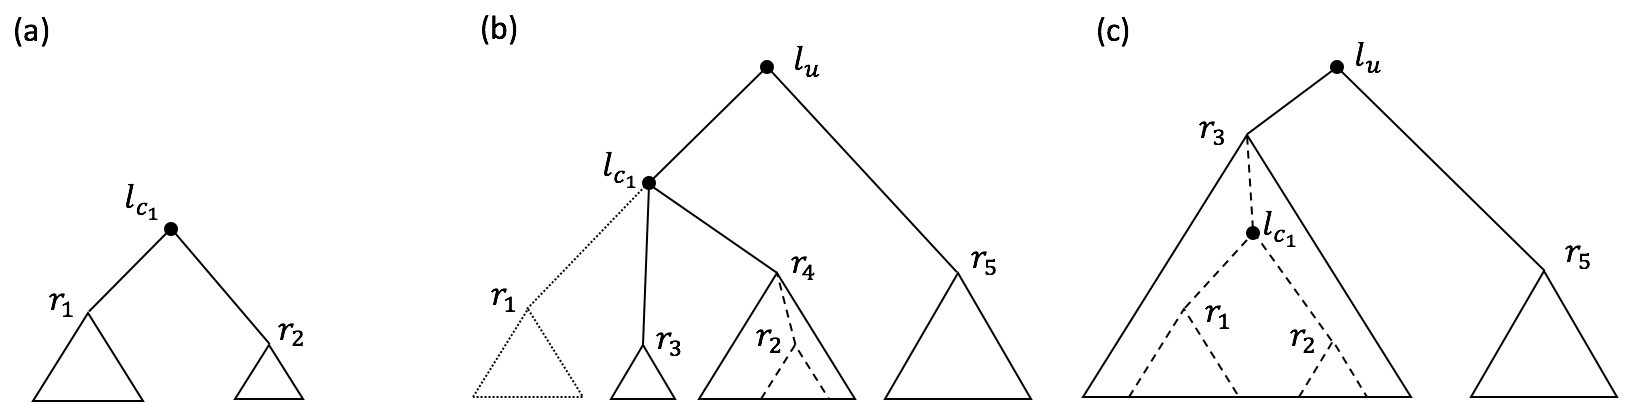
\includegraphics[scale=0.6]{incompatibilityrecursive}
        \centering
        \caption{}
        \label{fig:incompatibilityrecursive}
    \end{figure}

    Figure~\ref{fig:incompatibilityrecursive} illustrates two of of the interesting base cases for this process. Firstly, note that $minCover^{T}(C) = \{c_1, c_2\}$ and $minCover^{T}(C \cup \leafset^{T}(u)) = \{c_1, c_2, c_3\}$. The circled nodes belong to $incompatible^{T}(C)$, while nodes marked with a square belong to $incompatible^{T}(C \cup \leafset^{T}(u))$. Figure~\ref{fig:incompatibilityrecursive}(b) gives a case where $c_3$ is a descendant of $l_C$. In this case, we simply need to add the nodes in $path^{T}(c_3, l_C)$ to $incompatible^{T}(C)$ to give us $incompatible^{T}(C \cup \leafset^{T}(u))$. Figure~\ref{fig:incompatibilityrecursive}(b) gives a case where $c_3$ is not a descendant of $l_C$. In this case, we need add $path^{T}[l_C, l_{Cu})$ and $path^{T}(c_3, l_{Cu})$ to $incompatible^{T}(C)$.

    Observe that we also need to arrive at these base cases, we need to find the node $c_3 \in minCover^{T}(C \cup \leafset^{T}(u))$. This is done by falling the same recursive mechanism as in $addToCover$.
    \newline

    \begin{incompatibilityrecursive}
        \label{lem:incompatibilityrecursive}

        Given a tree $T$, a cluster $C \subseteq L$ and a node $u \in V(T)$ such that $\leafset^{T}(u) \cap C = \emptyset$, let $S = minCover^{T}(C)$, $I = incompatible^{T}(C)$, $l_C = lca^{T}(C)$ and $l_{Cu} = lca^{T}(C \cup \{u\})$. Let $v \in minCover^{T}(C \cup \leafset^{T}(u))$ such that $v$ is an ancestor of $u$. Define the operation \[updateIncompatible^{T}(I, u) = (I - path^{T}(u, v]) \cup path^{T}(v, l_{Cu}) \cup path^{T}(l_C, l_{Cu}) \cup
        \begin{cases}
            \{l_C\} & \leafset^{T}(l_C) \neq C \wedge l_C \neq l_{Cu}\\
            \emptyset & otherwise
        \end{cases}\]
        Then $updateIncompatible^{T}(I, u) = incompatible^{T}(C \cup \leafset^{T}(u))$.

        \begin{proof}
            Let the cluster $Cu$ be $C \cup \leafset^{T}(u)$. It can be seen from the structure of the $addToCover$ operation that $minCover^{T}(Cu) - minCover^{T}(C) = \{v\}$ and $minCover(C) - minCover^{T}(Cu) \subseteq V(T[v])$.

            $\longrightarrow$. Take any node $w \in updateIncompatible^{T}(I, u)$.

            Take the case where $w \in I - path^{T}(u, v]$. Since $w \in I$, there is some $c \in minCover^{T}(C)$ such that $w \in path^{T}(c, l_{C})$, by Lemma~\ref{lem:incompatibilitymincover}. If $c \not\in V(T[v])$, then $c \in minCover^{T}(Cu)$ and so $w \in incompatible^{T}(Cu)$. Otherwise, $c \in V(T[v])$. If $w$ is a proper ancestor of $v$, then $w \in incompatible^{T}(Cu)$. Otherwise, $w \in V(T[v])$. Since $w \in I - path^{T}(u, v]$, $w \not\in path^{T}(u, v]$, so $w$ is not an ancestor of $u$. Since $w \in incompatible^{T}(C)$, there is some leaf $x \in \leafset^{T}(w)$ such that $x \not\in C$. But also $x \not\in \leafset^{T}(u)$. Then $v \not\in minCover^{T}(Cu)$ because $x \in \leafset^{T}(v)$, which gives a contradiction, hence $w \not\in V(T[v])$.

            Otherwise, if $w \in path^{T}(v, l_{Cu})$, then $w \in incompatible^{T}(Cu)$ by Lemma~\ref{lem:incompatibilitymincover}.

            Otherwise, suppose $w \in path^{T}(l_C, l_{Cu})$. Then $C \subset \leafset^{T}(w)$. Also, $v$ is not a descendant of $w$, otherwise $w = l_{Cu}$. So $Cu - \leafset^{T}(w) \neq \emptyset$. Since $C \subset \leafset^{T}(w)$, there is some leaf $x \in \leafset^{T}(w)$ such that $x \not\in C$. Also, $x \not\in \leafset^{T}(u)$ since $v$ is not a descendant of $w$, so $x \not\in Cu$. Finally, $\leafset^{T}(w) \cap Cu \neq \emptyset$ because $C \subset \leafset^{T}(w)$ and $C \subset Cu$, thus $w \in incompatible^{T}(Cu)$.

            If none of the above are true, $w = l_C$ and $\leafset^{T}(l_C) \neq C$. Then

            If $w \not\in incompatible^{T}(Cu)$, then there is some node $c \in minCover^{T}(C)$ such that $c \not\in minCover^{T}(Cu)$ and $w \in path^{T}(c, l_{Cu})$. But then $c \in V(T[v])$. Also, $w$ is not a proper ancestor of $v$, otherwise $w \in incompatible^{T}(Cu)$, so $w \in V(T[v])$. Since $w \in incompatible^{T}(C)$, $w \not\in incompatible^{T}(Cu)$ and $C \subseteq Cu$, there is some leaf $x \in leafset^{T}(w)$ such that $x \not\in C$ and $x \in Cu$. Thus $x \in \leafset^{T}(u)$, and so $w$ is an ancestor of $u$. Further, $w \neq u$ since $\leafset^{T}(u) \cap C = \emptyset$ and so $w \not\in incompatible^{T}(C)$. Thus $w \in path^{T}(u, v]$, which leads to a contradiction.

            \textit{Case 1.} If $l_{Cu} = l_C$, then $u$ is a proper descendant of $l_C$.  We need to then show that $I - path^{T}(u, v] \cup path^{T}(v, l_{Cu}) = incompatible^{T}(Cu)$.

            $\longrightarrow$. Take any node $w \in I - path^{T}(u, v] \cup path^{T}(v, l_{Cu})$. If $w \in path^{T}(v, l_{Cu})$ then $w$ trivially belongs to $incompatible^{T}(Cu)$. Otherwise, $w \in I - path^{T}(u, v]$. If $w \not\in incompatible^{T}(Cu)$, then there is some node $c \in minCover^{T}(C)$ such that $c \not\in minCover^{T}(Cu)$ and $w \in path^{T}(c, l_{Cu})$. But then $c \in V(T[v])$. Also, $w$ is not a proper ancestor of $v$, otherwise $w \in incompatible^{T}(Cu)$, so $w \in V(T[v])$. Since $w \in incompatible^{T}(C)$, $w \not\in incompatible^{T}(Cu)$ and $C \subseteq Cu$, there is some leaf $x \in leafset^{T}(w)$ such that $x \not\in C$ and $x \in Cu$. Thus $x \in \leafset^{T}(u)$, and so $w$ is an ancestor of $u$. Further, $w \neq u$ since $\leafset^{T}(u) \cap C = \emptyset$ and so $w \not\in incompatible^{T}(C)$. Thus $w \in path^{T}(u, v]$, which leads to a contradiction.

            $\longleftarrow$. Take any node $w \in incompatible^{T}(Cu)$. If $w \in path^{T}(v, l_{Cu})$, then we are done. Otherwise, $w \in path^{T}(c, l_{Cu})$ for some $c \in minCover^{T}(Cu) - \{v\}$. Then $w \in I$, since $minCover^{T}(Cu) - \{v\} \subseteq minCover^{T}(C)$. Also, $w \not\in V(T[v])$ since $\leafset^{T}(v) \subseteq Cu$. Thus $w \in I - path^{T}(u, v]$.

            \textit{Case 2.}

            \textit{Case 3.} If $l_{Cu} = l_C$ and $\leafset^{T}(l_C) \neq C$, $minCover^{T}(Cu) = S \cup \{u\}$, since


            For the three base cases, $\leafset^{T}(v) \not\subseteq C \cup \leafset^{T}(u)$. By the same argument as in Lemma~\ref{lem:mincoverrecursive}, $minCover^{T}(C \cup \leafset^{T}(u)) = minCover^{T}(C) \cup \{u\}$. Note that $path(u, l_C) \subseteq path(u, l_{Cu})$, thus $I \cup path^{T}(u, l_{Cu}) = incompatible^{T}(C) \cup path^{T}(u, l_{Cu})$.

            \textit{Base Case 1.} $l_{Cu} = l_C$.

            We first show that $incompatible^{T}(C \cup \leafset^{T}(u)) \subseteq incompatible^{T}(C) \cup path^{T}(u, l_{Cu})$. Take any node $w \in incompatible^{T}(C \cup \leafset^{T}(u))$. If $w \in path^T(u, l_{Cu})$, then we are done. Otherwise, by Lemma~\ref{lem:incompatibilitymincover}, $w \in path^{T}(c, l_{Cu})$ for some node $c \in minCover^{T}(C \cup \leafset^{T}(u))$. But since $l_{Cu} = l_{C}$, $w \in incompatible^{T}(C)$.

            Now we show that $incompatible^{T}(C) \cup path^{T}(u, l_{Cu}) \subseteq incompatible^{T}(C \cup \leafset^{T}(u))$. Take any node $w \in incompatible^{T}(C) \cup path^{T}(u, l_{Cu})$. If $w \in path^{T}(u, l_{Cu})$, then $w \in incompatible^{T}(C \cup \leafset^{T}(u))$ by Lemma~\ref{lem:incompatibilitymincover} since $u \in minCover^{T}(C \cup \leafset^{T}(u))$. Otherwise, $w \in path^{T}(c, l_C)$ for some node $c \in minCover^{T}(C)$, by Lemma~\ref{lem:incompatibilitymincover}. Since $minCover^{T}(C) \subseteq minCover^{T}(C \cup \leafset^{T}(u))$ and $l_C = l_{Cu}$, $w \in incompatible^{T}(C \cup \leafset^{T}(u))$.

            \textit{Base Case 2.} $l_{Cu} \neq l_C \wedge\, \leafset^{T}(l_C) = C$. Note that since $\leafset^{T}(l_C) = C$, $minCover^{T}(C) = \{l_C\}$. Then by Lemma~\ref{lem:incompatibilitymincover}, $incompatible^{T}(C \cup \leafset^{T}(u)) = path^T(u, l_{Cu}) \cup path^{T}(l_C, l_{Cu})$. Since $incompatible^T(C) = \emptyset$, we are done.

            \textit{Base Case 3.} $l_{Cu} \neq l_C \wedge\, \leafset^{T}(l_C) \neq C$.

            We first show that $incompatible^{T}(C \cup \leafset^{T}(u)) \subseteq incompatible^{T}(C) \cup path^{T}(u, l_{Cu}) \cup path^{T}[l_C, l_{Cu})$. Take any node $w \in incompatible^{T}(C \cup \leafset^{T}(u))$. If $w \in path^T(u, l_{Cu})$, then we are done. Otherwise, by Lemma~\ref{lem:incompatibilitymincover}, $w \in path^{T}(c, l_{Cu})$ for some node $c \in minCover^{T}(C \cup \leafset^{T}(u))$. If $w$ is an ancestor of $l_C$, then $w \in path^{T}[l_C, l_{Cu})$, so we are done. Otherwise, if $w$ is a proper descendant of $l_C$, then $w \in path^{T}(c, l_C)$, so $w \in incompatible^{T}(C)$.

            Now we show that $incompatible^{T}(C) \cup path^{T}(u, l_{Cu}) \cup path^{T}[l_C, l_{Cu}) \subseteq incompatible^{T}(C \cup \leafset^{T}(u))$. Take any node $w \in incompatible^{T}(C) \cup path^{T}(u, l_{Cu}) \cup path^{T}[l_C, l_{Cu})$. By the same argument as in the first case, if $w \in incompatible^{T}(C) \cup path^{T}(u, l_{Cu})$, then $w \in incompatible^{T}(C \cup \leafset^{T}(u))$. Otherwise, $w \in path^{T}[l_C, l_{Cu})$. Then, since $\leafset^{T}(l_C) \neq C$, there is some node $c$ which is a proper descendant of $l_C$ such that $c \in minCover^T(C)$. Thus $w \in path^{T}(c, l_{Cu})$, so $w \in incompatible^{T}(C \cup \leafset^{T}(u))$.

            \textit{Inductive Case.} $\leafset^{T}(v) \subseteq C \cup \leafset^{T}(u)$. By the same argument as in Lemma~\ref{lem:mincoverrecursive}, $minCover^{T}(C - \leafset^{T}(v)) = minCover^{T}(C) - children(v)$. Then, it is clear that $incompatible^{T}(C - \leafset^{T}(v)) \subseteq I - \{v\} \subseteq incompatible^{T}(C - \leafset^{T}(v)) \cup path(v, l_{Cu})$. Thus, inductively, $updateIncompatible^{T}(I, u) = updateIncompatible^{T}(I - \{v\}, v) = incompatible^{T}(C - \leafset^{T}(v) \cup \leafset^{T}(v)) = incompatible^{T}(C \cup \leafset^{T}(u))$. Note that the recursion is well defined since in each recursive call, we go one node further up the tree.
        \end{proof}
    \end{incompatibilityrecursive}

    As done when computing the minimum cover, we implement the check for whether $\leafset^{T}(v) \subseteq C \cup \leafset^{T}(u)$ and $\leafset^{T}(l_C) = C$ using a counter property.

    This gives us the algorithm \texttt{Update\_Incompatible} which, for some tree $T$ and cluster $C \subseteq L$, takes in some node $u \in V(T)$, where $\leafset^{T}(u) \cap C = \emptyset$, a node $l_C = lca^{T}(C)$, a set $I \subseteq V(T)$ where $incompatible^{T}(C) \subseteq I \subseteq incompatible^{T}(C) \cup path(u, lca^T(C))$ and the tree $T$, where for each $w \in V(T)$, $counter(w) = |\{\leafset^{T}(c) \subseteq C : c \in children(w)\}|$. It returns $incompatible^{T}(C \cup \leafset^{T}(u))$, the node $l_{Cu} = lca^{T}(C \cup \{u\})$ and $T$, where for each $w \in V(T)$, $counter(w) = |\{\leafset^{T}(c) \subseteq C \cup \leafset^{T}(u) : c \in children(w)\}|$.

    \begin{algorithm}
        \caption{Update\_Incompatible}
        \label{alg:updateincompatible}

        \begin{algorithmic}[1]
            \Input For some tree $T$ and cluster $C \subseteq L$, takes in some node $u \in V(T)$, where $\leafset^{T}(u) \cap C = \emptyset$, the set $S = minCover^{T}(C)$, the set $I = incompatible^{T}(C)$, the node $l_C = lca^{T}(C)$ and the tree $T$, where for each $w \in V(T)$, $counter(w) = |\{\leafset^{T}(c) \subseteq C : c \in children(w)\}|$.

            \Output $minCover^{T}(C \cup \leafset^{T}(u))$, $incompatible^{T}(C \cup \leafset^{T}(u))$, the node $l_{Cu} = lca^{T}(C \cup \{u\})$ and $T$, where for each $w \in V(T)$, $counter(w) = |\{\leafset^{T}(c) \subseteq C \cup \leafset^{T}(u) : c \in children(w)\}|$.

            \State $S, v :=$ \texttt{Add\_To\_Cover}$(S, u, T)$

            \State $l_{Cu} := lca^T(l_C, u)$

            \State $I := (I - path^{T}(u, v]) \cup path^{T}(v, l_{Cu}) \cup path^{T}(l_C, l_{Cu})$

            \If{$counter(l_C) = |children(l_C)|$}
                \State \Return $S,\, I,\, l_{Cu},\, T$
            \Else
                \State \Return $S,\, I \cup \{l_C\},\, l_{Cu},\, T$
            \EndIf
        \end{algorithmic}
    \end{algorithm}

    We now develop the solution for \texttt{Filter\_Clusters}. Recall that this method takes trees $\TA$ and $\TB$ as input. First, for any node $u \in V(\TA)$, define $incompatible^{\TB}(u)$ to be $incompatible^{\TB}(\leafset^{\TA}(u))$. As discussed earlier, the idea is to find $incompatible^{\TB}(u)$ for each node $u \in V(\TA)$. To do so, we recursively obtain $incompatible^{\TB}(c)$, where $c$ is the heavy child of $u$. We also get $minCover^{\TB}(c')$ for each $c' \in$ side children of $u$. Then for $v \in \bigcup_{c' \in \text{side children of } u} minCover^{\TB}(c')$ we use $updateIncompatible$ to insert $v$ into $incompatible^{\TB}(c)$, giving us $incompatible^{\TB}(u)$. Thus, it would be helpful if \texttt{Filter\_Clusters} returned $incompatible^{\TB}(u)$ and $minCover^{\TB}(u)$.

    {\color{red} Should I give the \texttt{Filter\_Clusters} algorithm first?}

    This leads to defining the helper function \texttt{Filter\_Clusters\_Helper}, which takes as input $u \in V(\TA)$ and $\TB$ and returns $incompatible^{\TB}(\leafset^{\TA}(u))$, $minCover^{\TB}(\leafset^{TA}(u))$, a copy of $\TA[u]$ where for any node $w \in \TA[u]$, $w$ is marked for deletion iff $\weight(w) \leq \weight(v)$ for any $v \in V(\TB)$ with $u \not\compatible v$ and $\TB$ where for each $v \in V(\TA)$, $counter(v) = |\{\leafset^{\TB}(c) \subseteq \leafset^{\TA}(u) : c \in children(v)\}|$. The third item is used to keep track of which nodes in $\TA$ need to be deleted. The last item is $\TB$ with counter values updated, so that we can use it while updating the set of incompatible nodes.

    Then \texttt{Filter\_Clusters} can simply take the copy of $\TA$ output by \texttt{Filter\_Clusters\_Helper}$(root(\TA), \TB)$ and delete the marked nodes in a top-down traversal. The resulting algorithm is shown below. Note that it also does some preprocessing on $\TB$, which is explained in more detail below.

    \begin{algorithm}
        \caption{Filter\_Clusters}
        \label{alg:filterclusters}

        \begin{algorithmic}[1]
            \Input Trees $\TA$ and $\TB$ with $\leafset^{\TA} = \leafset^{\TB} = L$ where every cluster has a known $weight$.

            \Output A tree $T$ where $\mathcal{C}(T) = \{C : C \in \mathcal{C}(\TA) \text{ and } \weight(C) > max(\{\weight(C_1) : C_1 \in \mathcal{C}(\TB) \text{ and } C_1 \not\compatible C\})\}$ and $\leafset^T = L$

            \State Preprocess $\TB$ for lca, $cFD$ and $rmqTree$ queries and compute $|children(w)|$ for each node $w \in V(\TB)$

            \State $\_, \_, \TA, \_ :=$ \texttt{Filter\_Clusters\_Helper}$(root(\TA), \TB)$

            \State Do a top-down traversal of $\TA$, deleting all marked nodes

            \State \Return $\TA$
        \end{algorithmic}
    \end{algorithm}

    Now we need to develop \texttt{Filter\_Clusters\_Helper}. The key to this running fast is ensuring that when we recursively call the function on a side child $c'$ of some node $u \in V(\TA)$, we restrict $\TB$ such $\leafset^{\TB} = \leafset^{\TA}(c')$. Let $\tau = \TA[c']$. We reuse the technique described in \cite{jansson2018algorithms}. We wish to construct a tree $\TB||\leafset^{\tau}$ such that $\leafset^{\TB||\leafset^{\tau}} = \leafset^{\tau}$, but at the same time does not lose important weight information. To do so, we first construct $\TB|\leafset^{\tau}$ and let weight of each node in this tree be the same as its weight in $\TB$. For each non-root node $u \in V(\TB|\leafset^{\tau})$, let $v = parent^{\TB|\leafset^{\tau}}(u)$, then if $path^{\TB}(u, v) \neq \emptyset$, we create a new node $z$ in $\TB|\leafset^{\tau}$, set $parent(u) = z$ and $parent(z) = v$. Also, we set $\weight(z) = max_{w \in path^{\TB}(u, v)} \weight(w)$. Note that this value can be obtained with an $rmqTree^{\TB}[parent(u), cFD(v)]$ query, which we denote by $rmqTree^{\TB}(u, v)$. This gives us the tree $\TB||\leafset^{\tau}$.

    Further, for any node $u \in V(\TB||\leafset^{\tau})$, if $\leafset^{\TB||\leafset^{\tau}}(u) \neq \leafset^{\TB}(u)$, then $u$ is marked as $spoiled$. Special nodes are all marked as $spoiled$, since it is certain that the nodes they represent do not have their full leafset in $\TB||\leafset^{\tau}$. Observe that the ancestor of any spoiled node is also spoiled. Figure~\ref{fig:specialnodes} illustrates this entire process.

    \begin{figure}[h]
        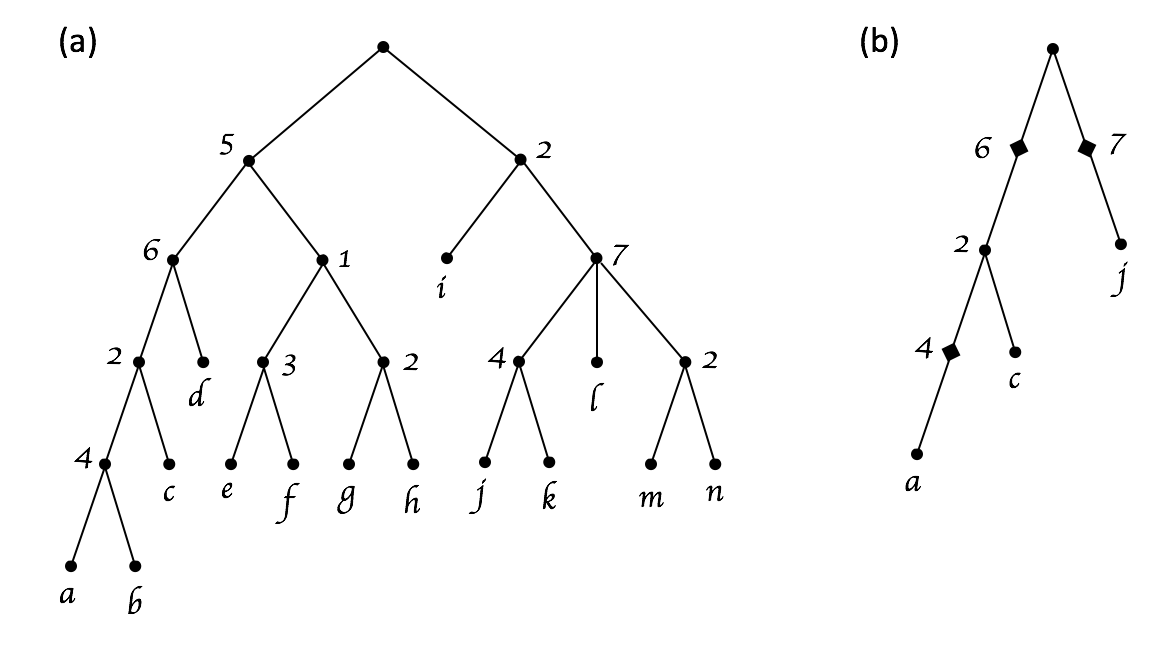
\includegraphics[scale=0.5]{specialnodes}
        \centering
        \caption{Part (a) shows a tree $T$ where all internal nodes are labelled with their weights. Part (b) shows the tree $T||\{a, c, j\}$. Again, internal nodes are labelled with their weights. Nodes represented by diamonds in this figure are special nodes. Observe that the special node that is a parent of the leaf $j$ has weight $7$ since the nodes on the path from $j$ to the root of $T$ had weights $4, 7$ and $2$. Also note that all internal nodes in (b) are spoiled.}
        \label{fig:specialnodes}
    \end{figure}

    Since we now have spoiled nodes, this means that when running \texttt{Add\_To\_Cover} or \texttt{Update\_Incompatible}, our $counter$ check is not good enough, as for some node $u \in V(\TB||\leafset^{\tau})$, even if $\leafset^{\TB||\leafset^{\tau}}(u) \subseteq C$, where $C$ is some cluster under consideration, that does not guarantee that $\leafset^{\TB}(u) \subseteq C$. Thus we need to expand our check to include the condition that $u$ must not be spoiled.

    This leads to the algorithm \texttt{Update\_Incompatible\_Spoiled}. This algorithm combines \texttt{Add\_To\_Cover} and \texttt{Update\_Incompatible} along with the concept of spoiled nodes. For some tree $T$ and cluster $C \subseteq L$, the algorithm takes in a node $u \in V(T)$, where $\leafset^{T}(u) \cap C = \emptyset$, a node $l_C = lca^{T}(C)$, the set $S = minCover^{T}(C)$, a set $I \subseteq V(T)$ where $incompatible^{T}(C) \subseteq I \subseteq incompatible^{T}(C) \cup path(u, lca^T(C))$ and the tree $T$, where for each $w \in V(T)$, $counter(w) = |\{\leafset^{T}(c) \subseteq C : c \in children(w)\}|$. It returns $minCover^{T}(C \cup \leafset^{T}(u))$, $incompatible^{T}(C \cup \leafset^{T}(u))$, the node $l_{Cu} = lca^{T}(C \cup \{u\})$ and $T$, where for each $w \in V(T)$, $counter(w) = |\{\leafset^{T}(c) \subseteq C \cup \leafset^{T}(u) : c \in children(w)\}|$.

    \begin{algorithm}
        \caption{Update\_Incompatible\_Spoiled}
        \label{alg:updateincompatiblespoiled}

        \begin{algorithmic}[1]
            \Input For some tree $T$ and cluster $C \subseteq L$, takes in some node $u \in V(T)$, where $\leafset^{T}(u) \cap C = \emptyset$, a node $l_C = lca^{T}(C)$, the set $S = minCover^{T}(C)$, a set $I \subseteq V(T)$ where $incompatible^{T}(C) \subseteq I \subseteq incompatible^{T}(C) \cup path(u, lca^T(C))$ and the tree $T$, where for each $w \in V(T)$, $counter(w) = |\{\leafset^{T}(c) \subseteq C : c \in children(w)\}|$.

            \Output $minCover^{T}(C \cup \leafset^{T}(u))$, $incompatible^{T}(C \cup \leafset^{T}(u))$, the node $l_{Cu} = lca^{T}(C \cup \{u\})$ and $T$, where for each $w \in V(T)$, $counter(w) = |\{\leafset^{T}(c) \subseteq C \cup \leafset^{T}(u) : c \in children(w)\}|$.

            \State $v := parent(u)$

            \State $counter(v) := counter(v) + 1$

            \State $l_{Cu} := lca^T(l_C, u)$

            \If{$counter(v) = |children(v)|$ and $v$ is not spoiled}
                \State \Return \texttt{Update\_Incompatible\_Spoiled}$(v, l_{Cu}, S - children(v), I - v, T)$
            \ElsIf{$l_{Cu} = l_C$}
                \State \Return $S \cup \{u\}, I \cup path^{T}(u, l_{Cu}), l_{Cu}, T$
            \ElsIf{$counter(l_C) = |children(l_C)|$}
                \State \Return $S \cup \{u\}, I \cup path^{T}(u, l_{Cu}) \cup path^{T}(l_C, l_{Cu}), l_{Cu}, T$
            \Else
                \State \Return $S \cup \{u\}, I \cup path^{T}(u, l_{Cu}) \cup path^{T}[l_C, l_{Cu}), l_{Cu}, T$
            \EndIf
        \end{algorithmic}
    \end{algorithm}

    Also note we now have an explanation for the preprocessing done on $\TB$ in \texttt{Filter\_Clusters}. $lca$ queries are needed in \texttt{Update\_Incompatible\_Spoiled}, while $cFD$ and $rmqTree$ queries are needed to construct the trees $\TB||\leafset^{\tau}$.

    With the procedure \texttt{Update\_Incompatible\_Spoiled} in hand, we can now write \texttt{Filter\_Clusters\_Helper}, presented in Algorithm~\ref{alg:filterclustershelper}.

    \begin{algorithm}
        \caption{Filter\_Clusters\_Helper}
        \label{alg:filterclustershelper}

        \begin{algorithmic}[1]
            \Input For some trees $\TA$ and $\TB$, takes in some node $u \in V(\TA)$ and $\TB$, where $\leafset^{\TA}(u) \subseteq \leafset^{\TB}$.

            \Output $incompatible^{\TB}(\leafset^{\TA}(u))$, $minCover^{\TB}(\leafset^{TA}(u))$, a copy of $\TA[u]$ where for any node $w \in \TA[u]$, $w$ is marked for deletion iff $\weight(w) \leq \weight(v)$ for any $v \in V(\TB)$ with $u \not\compatible v$ and $\TB$ where for each $v \in V(\TA)$, $counter(v) = |\{\leafset^{\TB}(c) \subseteq \leafset^{\TA}(u) : c \in children(v)\}|$.

            \State $c := $ heavy child of $u$

            \State $T_u :=$ tree consisting of only a root

            \State $incompatible, minCover, T_{c}, \TB :=$ \texttt{Filter\_Clusters\_Helper}$(c, \TB)$

            \ForAll{$c' \in$ side children of $u$}
                \State Construct $\TB||\TA[c']$

                \State Preprocess $\TB||\TA[c']$ for lca queries and compute $|children(w)|$ for each node $w \in V(\TB||\TA[c'])$

                \State $\_, minCover_{c'}, T_{c'}, \_ :=$ \texttt{Filter\_Clusters\_Helper}$(c', \TB||\TA[c'])$

                \State Attach the root of $T_{c'}$ to the root of $T_u$

                \ForAll{$v \in minCover_{c'}$}
                    \State $incompatible, minCover, \TB :=$ \texttt{Update\_Incompatible\_Spoiled}$(incompatible, minCover, v, \TB)$
                \EndFor
            \EndFor

            \IIEf{$incompatible$ is empty}
                {$M := 0$}
                $M :=$ maximum weight of a node in $incompatible$

            \IIf{$\weight(u) \leq M$}
                mark root of $T_u$ for deletion

            \State \Return $incompatible, minCover, T_u, \TB$
        \end{algorithmic}
    \end{algorithm}

%             We preprocess $\TB$ for \textit{lca} queries using the technique of \cite{bender2000lca}. This takes $O(n)$ preprocessing time and thereafter allows us to answer \textit{lca} queries in $O(1)$ time. $\TB$ is also preprocessed to create the cFL and RMQ data structures using Lemma~\ref{lem:rmqdatastructure} and~\ref{lem:cfddatastructure}. These take $O(n\,log\,n)$ preprocessing time and thereafter allow us to answer $rmqTree$ queries in $O(1)$ time. The bottom-up traversal of $\TB$ to compute $|children(v)|$ for all $v \in V(\TB)$ takes $O(n)$ time. Finally, copying $\TA$ takes $O(n)$ time.
%
%             As before, we use linked lists to implement sets of nodes, coupled with membership properties.
%
%             The data structure used for $incompatible$ is the Brodal queue of \cite{brodal1995fast}. This allows $insert$ and $findMax$ operations in $O(1)$ time and $delete$ in $O(log\,m)$ time (where $m$ is the number of elements in the queue). Since the number of nodes in $\TB$ is $O(n)$, the number of elements in the queue is always $O(n)$ and so deletions cost $O(log\,n)$ time.
%
%             Let $m = |\leafset^{\TA}|$ for some call to \texttt{Filter\_Clusters\_Helper}$(\TA, \TB)$. Recall that $n = |\leafset^{\TB}|$. Observe that for any cluster $C$, $|RST^{\TB}(C)| \leq |C|$. Thus $|boundary^{\TB}(p_i)| \leq |\leafset^{\TA}(p_i) - \leafset^{\TA}(p_{i-1})|$ and $\sum_{i = 2}^{\gamma} |boundary^{\TB}(p_i)| \leq m$. It can also be seen that $\sum_{P_i \in \mathcal{P}(\TA), p_j \in P_i} removedRST(p_j, p_{j-1}) \leq |V(\TA)|$.
%
%             Computing the centroid path takes $O(m)$ time. Constructing the $boundary$ sets costs $O(m)$ time in total. Since $lca$ queries can be made in constant time and the total number of $lca$ queries is $O(m)$, this also costs $O(m)$ time.
%
%             The runtime of \texttt{Compute\_Roots\_Of\_Subtrees} is $O(|boundary^{\TB}(p_i)| + |removedRST^{\TB}(p_i, p_{i-1})|)$. The cost due to the first half of this expression is $O(m)$. The cost due to the second half of this expression is $O(n)$ over all calls to \texttt{Filter\_Clusters\_Helper}.
%
%             $O(m)$ insertions are made into $incompatible$, costing $O(m)$ time. Since the total size of all the removed sets is $O(n)$, there are a total of $O(n)$ deletions from $incompatible$ over all calls due to Step~\ref{step:removedrootsremoval}. Step~\ref{step:oldrootremoval} also causes a total of $O(n)$ deletions over all calls as this step happens once for each node in the centroid path, and every node in $\TA$ belongs to exactly one centroid path. Thus deletions cost a total of $O(n\,log\,n)$ time.
%
%             We can hence write a recurrence for \texttt{Filter\_Clusters\_Helper} (ignoring steps that are being analysed over the entire call to \texttt{Filter\_Clusters}) in the following manner: $T(m) = \sum_{\tau \in \sigma(T)}T(|\leafset^{\tau}|) + O(m)$. Since for any $\tau \in \sigma(T)$, $|\leafset^{\tau}| \leq m/2$, there are $log\,m$ recursion levels, we get $T(n) = O(n\,log\,n)$.
%
%             Finally, we note that it takes $O(n)$ time to process $T_{\alpha'}$ after \texttt{Filter\_Clusters\_Helper} is done. This is because deleting all marked nodes can be done in a top down traversal (using the \texttt{delete} operation described in Subsection~\ref{subsec:delete}), where every node's parent changes at most once. Further, recall that the total preprocessing time is $O(n\,log\,n)$ and the time set aside to be analysed over the entire call to \texttt{Filter\_Clusters} is $O(n\,log\,n)$. Thus, \texttt{Filter\_Clusters} runs in $O(n\,log\,n)$ time.

    \section{Constructing the FDCT}
    \label{sec:freqdiffconstruction}

    \begin{freqdiffruntime}
        \label{theorem:freqdiffruntime}

        Given a set $\mathcal{S}$ of $k$ trees with identical leafsets of size $n$, the algorithm \texttt{Frequency\_Difference}$(\mathcal{S})$ runs in $O(kn\,log\,n)$ time.

        \begin{proof}
            By Corollary~\ref{cor:freqdiffruntimecomponents} and Lemmas~\ref{lem:weightingruntime} and~\ref{lem:filterclustersruntime}, \texttt{Frequency\_Difference} runs in $O(kn\,log\,n + k \cdot n\,log\,n) = O(kn\,log\,n)$ time.
        \end{proof}
    \end{freqdiffruntime}

    \newpage
    \bibliographystyle{plain}
    \bibliography{interim_report}
\end{document}
